\documentclass[uplatex]{jsarticle}
\AtBeginDvi{\special{pdf:mapfile dlbase14.map}}
\usepackage[dvipdfmx]{graphicx}
\usepackage{ascmac}
\usepackage{url}
\usepackage{plext}
\usepackage{listings,jlisting}

\lstset{language=c,%
  basicstyle=\ttfamily\scriptsize,%
  commentstyle=\textit,%
  classoffset=1,%
  keywordstyle=\bfseries,%
  frame=tRBl,%
  framesep=5pt,%
  showstringspaces=false,%
  numbers=left,%
  stepnumber=1,%
  numberstyle=\tiny,%
  tabsize=2%
}
\begin{document}

\title{EDAツールを用いた論理回路設計}
\author{名古屋大学工学部電気電子・情報工学科情報コース\\酒井 英伸(学籍番号081330766)\\sakai.hidenobu@f.mbox.nagoya-u.ac.jp}
\date{2016/10/6, 13}
\maketitle

\tableofcontents


\clearpage
%===================================================================
\section{はじめに}
%===================================================================

今回の実験では、ハードウェア記述言語であるVerilog HDLを用いて、設計を行う。また、そのコードの機能レベルの
シミュレーションや論理合成をソフトウェア上で行い、回路の動作検証、評価は実験1に関しては、書き換え可能な論理素子
であるFPGA(Field Programmable Gate Array)を使用した。

%===================================================================
\section{2入力1出力セレクタ回路の設計と動作実験(実験1)}
%===================================================================

%---------------------------------------------------------------------
\subsection{目的・概要}
%---------------------------------------------------------------------

この実験では、2入力1出力セレクタ回路の回路の設計と動作実験を行う。また、その機能レベルシミュレーションや
論理合成を行うための環境設定や、ソフトウェアの使い方を理解するとともに、書き換え可能な論理素子であるFPGA
を搭載した実験基盤を用いて、FPGA上に設計した回路を実現することを目的とする。。

%---------------------------------------------------------------------
\subsection{実験手順}
%---------------------------------------------------------------------

はじめに、以下の手順で今回の実験を行うためのコンピュータの環境は以下のとおりである。

\begin{itemize}
  \item OS: Linux
  \item Kernel: 2.6.32-642.6.1.el6.x86\_64
\end{itemize}

%----------------------------------
\subsubsection{EDAツールの環境設定}
%----------------------------------

\begin{enumerate}
  \item
    端末上で「{\tt ln -s /pub1/jikken/eda3/cadsetup.csh.altera path/to/directory}」
    \fontnote{lnコマンドはファイルやディレクトリへのリンクを作成するコマンド.}
    と入力して、ファイルのシンボリックリンク
    \fontnote{lnコマンドに-sオプションを指定することで、作成される。特定のファイルやディレクトリを指し示す別のファイルを作成して、それを通じて本体を三章できるようにする仕組みのこと.}
    を自分の作業用のディレクトリに作成した。
  \item 
    作成した設定ファイルを読み込むために「\tt source /path/to/directory/cadsetup.csh.altera}」
    \footnote{指定したファイルを読み込む.}
    と入力した。(この操作は端末を起動する度に実行する。)
\end{enumerate}

%----------------------------------
\subsubsection{Verilog HDLによる回路記述}
%----------------------------------

今回の実験では図\ref{fig:1}のような2入力1出力セレクタ回路を設計した。
仕様は以下の通りであった。

\begin{itemize}
  \item 入力: データD0, D1(それぞれ1ビット), セレクト信号S1(1ビット)
  \item 出力: データY(1ビット)
  \item 機能: セレクト信号S1の値が0か1かにより、データD0, D1の値をYに出力
  \item 図\ref{fig:1}はこのセレクタ回路の回路図と真理値表である。
\end{itemize}

\begin{figure}[htb]
  \begin{center}
    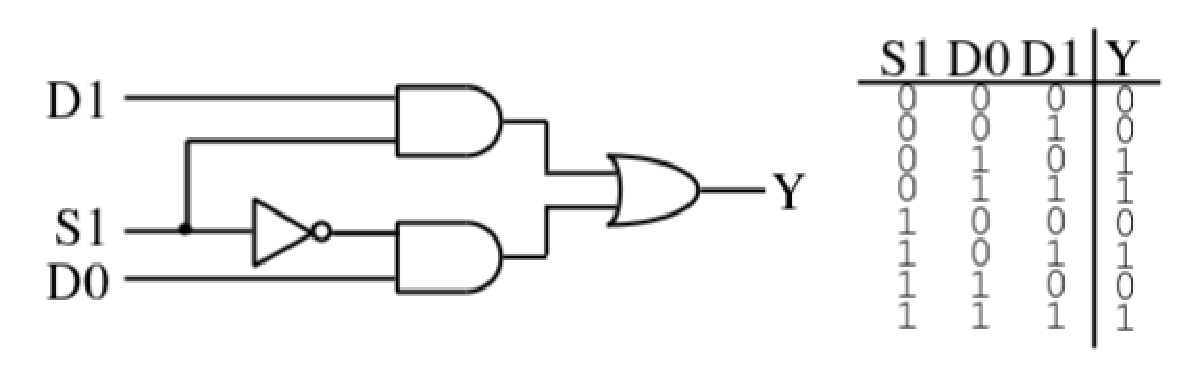
\includegraphics[width=13cm]{images/fig01.eps}
    \caption{2入力1出力セレクタ回路の回路図と真理値表}
    \label{fig:01}
  \end{center}
\end{figure}

まずは、2入力1セレクタ回路の記述を行った。
ソースコードは以下のようになった。

\lstinputlisting[caption=セレクタ回路,label=mux21.v]{../../jikken1/mux21.v}

このコードの説明を以下に記述する。

\begin{itemize}
  \item 1~5行目はコメントである。
  \item VerilogHDLでは、モジュールで一つの回路を記述するため、{\tt module ... endmodule}という記述をした。
  \item 7行目でモジュール名{\tt mux21} を定義して、ポート(入出力インタフェース)を( ... )内に記述した。
  \item 8, 9行目で各ポートの型(入力、出力、ビット数)を宣言した。
  \item 11行目は12行目の式のコメントである。
  \item 
    12行目で{\tt assign}文で、出力Yに論理式$(\lnot S_1 \land D_0) \lor (S_1 \land D_1)$を対応させた。この論理式は、図\ref{fig:1}の真理値表に対応している。
    {\tt assign}文は、シミュレーションの最中に、右辺のオブジェクトの値に変化が生じる度に実行される。
\end{itemize}

回路の設計をするには回路そのもの記述の他に、その記述した回路が正しく動作するかのテストの記述が必要となる。
これをテストベンチといい、今回の{\tt mux21.v}も同様にセレクタ回路の動作を確認するためのテストベンチ、{\tt test\_mux21.v}を作成した。

\lstinputlisting[caption=セレクタ回路のテストベンチ,label=test_mux21.v]{../../jikken1/test_mux21.v}

このコードも同様に説明を以下に記述する。   

\begin{itemize}
  \item 1~4行目はコメントである。
  \item 6行目で、シミュレーションの単位時間と精度を宣言した。今回はどちらも1nsと宣言した。
  \item 7行目で、mux21.vを取り込む記述をした。
  \item 9行目の {\tt module}以降で、テストベンチモジュールの宣言を行っている。
  \item 12行目で信号を与える入力ポートを指定した。
        {\tt reg}は記憶素子を表すオブジェクトである。
  \item 15行目で信号値を観測する出力ポートを指定した。
        {\tt wire}は配線を表すオブジェクトで、下位階層の出力ポートに接続しているオブジェクトを{\tt wire}宣言する。
  \item 20行目 ~ 34行目でテストパタンを宣言した。
        このテストパタンでは送る信号を表\ref{tab:1}にまとめた。また、図\ref{fig:1}の真理値表に基づいて、予想される出力Yの値も記述した。
\end{itemize}

\begin{table}[htb]
  \begin{center}
    \caption{test\_mux21.vによるテストパタン}
    \begin{tabular}{c|ccc|c} \hline
            & S1 & D0 & D1 & 予想される出力Y \\ \hline \hline
      初期値   & 0 & 0 & 0 & 0 \\
      20ns後  & 0 & 1 & 0 & 1 \\
      40ns後  & 1 & 1 & 0 & 0 \\
      60ns後  & 0 & 0 & 0 & 0 \\
      160ns後 & \multicolumn{3}{c|}{終了} & 0 \\ \hline
    \end{tabular}
    \label{tab:1}
  \end{center}
\end{table}

%----------------------------------
\subsubsection{機能レベルシミュレーション}
%----------------------------------

Verilog HDLで記述した回路が,機能的に正しく動作するかどうかを調べるために,論理シミュレータを用いた。
論理シミュレータには,Altera社のModelSim version 10.1d を用いた。
以下の手順で機能レベルシミュレーションを行った。

\begin{enumerate}
  \item 「{\tt vsim test\_mux21.v &}」コマンドを端末上で実行して、ModelSimでtest\_mux21.vを開いた。
  \item ModelSimのコンソールで「{\tt vlib work}」を実行して、ライブラリを作成した。
  \item 
    次に、「{\tt vlog test\_mux21.v}」コマンドを実行して、VerilogHDLで記述されたファイルのコンパイルを行った。
    この時、コンソール上で正しくコンパイルできた場合に表示される「{\tt Top level modules: test}」というメッセージを確認した。
  \item 最上位モジュールを読み込むために「{\tt vsim test}」を十個浮いて、コンパイルしたVerilogHDL記述内の最上位モジュールを読み込む。
  \item 次に、波形ウィンドウを「{\tt view wave}」コマンドで表示して、全ての入出力ポートの波形を表示する設定を「{\tt add wave *}」コマンドで行った。
  \item 最後に「{\tt run 80ns}」とコンソールに入力して、シミュレーションを開始し、その結果の波形を得た。
\end{enumerate}

%----------------------------------
\subsubsection{論理合成}
%----------------------------------

論理合成で、ハードウェア記述言語によって記述された回路を最適化して、ゲートレベルの記述であるネットリストに変換する。
論理合成には、FPGA設計フローにおける論理合成からFPGAマッピングまでの機能をサポートしているFPGA用統合開発ソフトウェアの
Quartus II Web Edition version 13.0.1を用いた。以下の手順で論理合成を行った。

\begin{enumerate}
  \item あらかじめ情報工学部実験用のサイトに上がっていたmux21.qpfをダウンロードした。
  \item 端末から「{\tt quartus &}」を実行してQuartus IIを起動して、プロジェクトファイルmux21.qpfを開いた。
        この時、Project Navigator1ウィンドウのEntity部分にコンパイル対象のFPGAとモジュールの名称(mux21~が表示されていることを確認した。
  \item ProcessingタブのStart Compilationでコンパイルを実行した。コンパイルが完了されると、メッセージウィンドウが開いてエラーが表示されていないことを確認した。
  \item コンパイル結果の確認を行った。Technology Map Viewerを用いて、咲いて季語の回路構成の確認や、Flow Summaryのロジックエレメントの確認をした。
        また、TImeQuest Timing Analyzerを用いて回路の遅延時間を確認した。
\end{enumerate}

%----------------------------------
\subsubsection{FPGAボードでの動作実験}
%----------------------------------

機能レベルシミュレーション、論理合成を行ったので、FPGAマッピングをするために、端末上で論理合成、レイアウト、FPGAマッピングの各機能を実行する一連の処理をまとめて実行した。
こkでのコンパイルはCUIで行い、「{\tt Quartus II Full Compilation was successful.}」と表示され、コンパイルが成功していることを確認した。
また、ディレクトリにmux.sofが生成されていることを確認した。

次に、以下の手順でAltera DE2-115ボードにsofファイルをインストールした。

\begin{enumerate}
  \item DE2-115ボードのマシンをUSBケーブルで接続した。また、DE2-115ボードに電源を入れるために電源を供給する専用のACアダプタを接続して、電源を入れた。
  \item 端末で「{\tt dmesg}」と入力して、マシンがボードを認識していることを確認した。
  \item ダウンロード用の設定ファイルmux21.cdfを作業ディレクトリに置いて、端末で「{\tt quartus\_pgm mux21.cdf}」と実行した。
        「{\tt Quartus II 32 bit Programmer was successful.}」と表示されたのを確認した。
  \item ボード上で、論理回路が仕様どおりに動作するかを確認した。表\ref{tab:1}に示した順に、スイッチやボタンを切り替え流れLEDの点灯の様子を記録した。
\end{enumerate}

%---------------------------------------------------------------------
\subsection{実験結果}
%---------------------------------------------------------------------

%----------------------------------
\subsubsection{機能レベルシミュレーション}
%----------------------------------

図\ref{fig:02}に示す波形を得た.

\begin{figure}[htb]
  \begin{center}
    \includegraphics[width=13cm]{images/fig02.eps}
    \caption{機能レベルシミュレーションを行った結果の波形}
    \label{fig:02}
  \end{center}
\end{figure}

%----------------------------------
\subsubsection{論理合成}
%----------------------------------

最適化後の回路構成は,図\ref{fig:03}のようになった.

\begin{figure}[htb]
  \begin{center}
    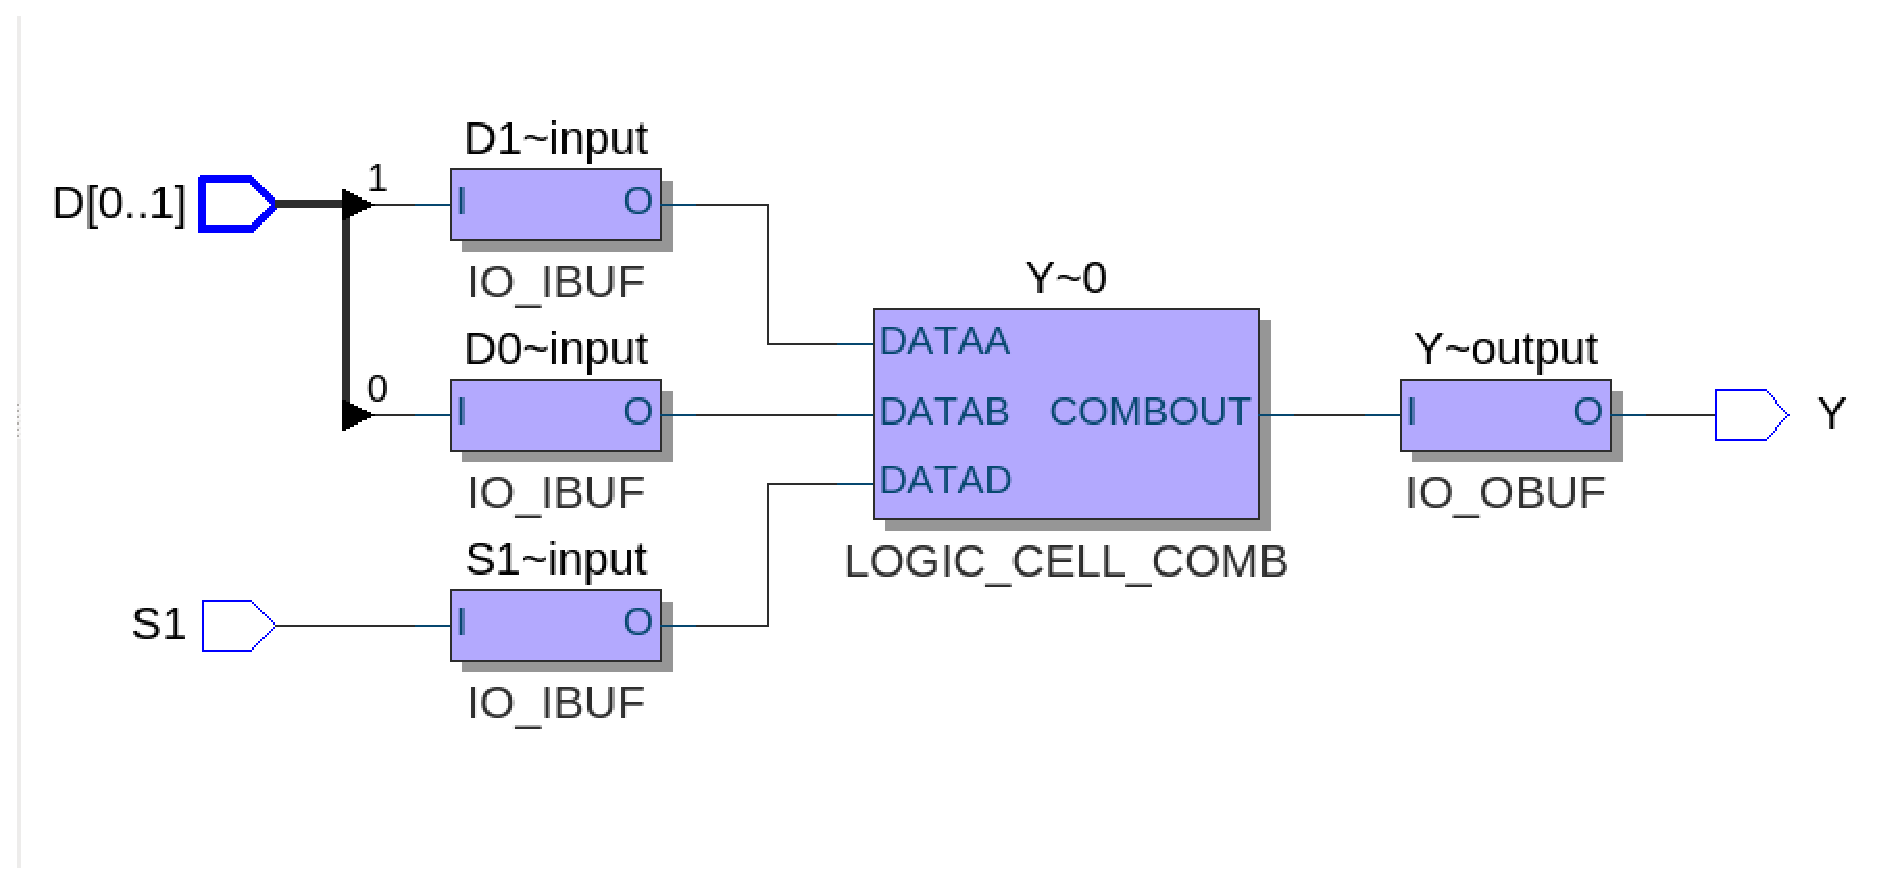
\includegraphics[width=13cm]{images/fig03.eps}
    \caption{最適化後の回路構成}
    \label{fig:03}
  \end{center}
\end{figure}

コンパイル結果のロジックエレメント数は図\ref{fig:04}のようだった. 
ロジックエレメント数は図\ref{fig:04}のTotal Logic Elementの部分である。

\begin{figure}[htb]
  \begin{center}
    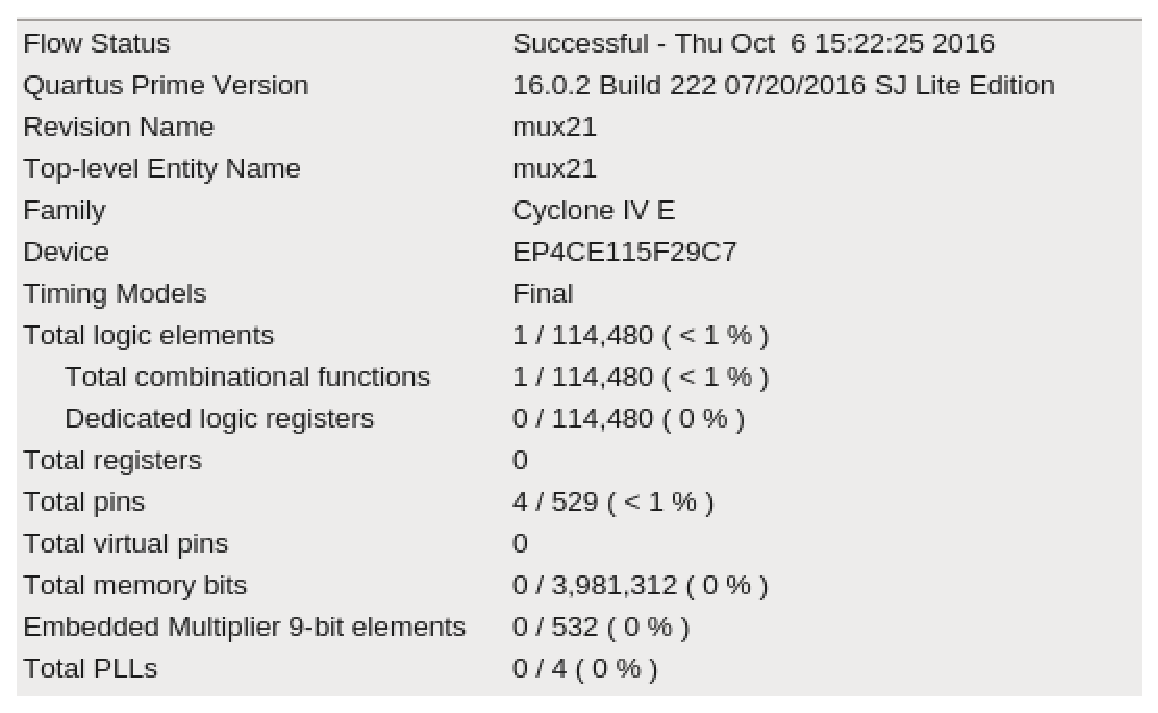
\includegraphics[width=10cm]{images/fig04.eps}
    \caption{ロジックエレメント数}
    \label{fig:04}
  \end{center}
\end{figure}

回路の遅延時間は図\ref{fig:05}の通りだった.
トータルの遅延時間はここでは、13.447nsとなる。

\begin{figure}[htb]
  \begin{center}
    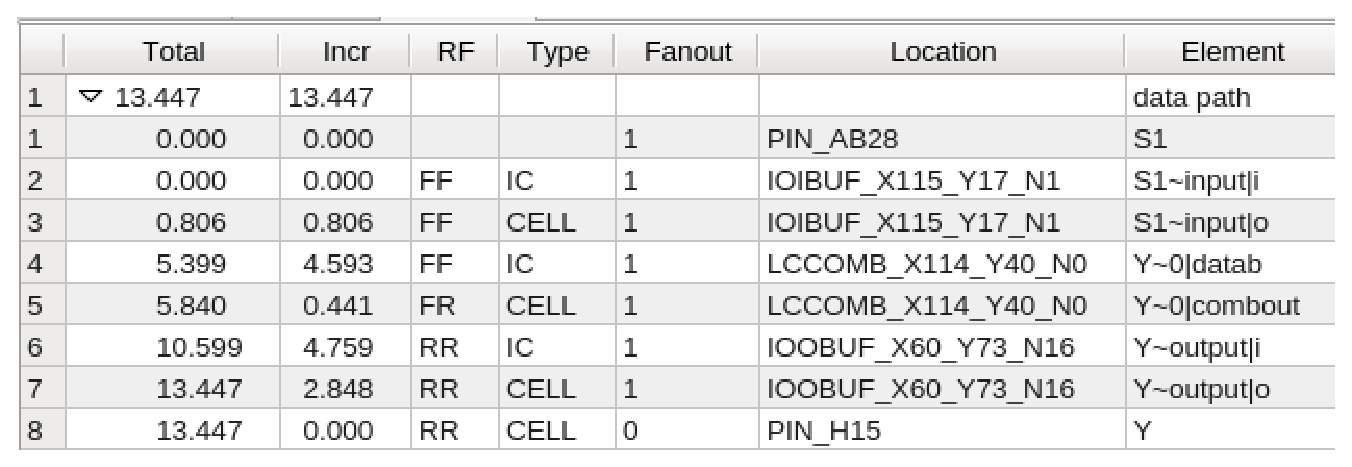
\includegraphics[width=10cm]{images/fig05.eps}
    \caption{遅延時間}
    \label{fig:05}
  \end{center}
\end{figure}

%----------------------------------
\subsubsection{FPGAボードでの動作実験}
%----------------------------------

表\ref{tab:1}で示したものと同じ結果になった.

\clearpage

%---------------------------------------------------------------------
\subsection{考察}
%---------------------------------------------------------------------

%----------------------------------
\subsubsection{機能レベルシミュレーション結果に対する評価}
%----------------------------------

図\ref{fig:02}の波形は、入力した値から、0の時は波形の下方、1の時は波形の情報で示されていることが推察される。
図\ref{fig:02}の{\tt /test\_mux21/Y}の波形に注目すると、表\ref{tab:1}で予想したYの出力値と一致している。
\bou{テストパターンに大して}、論理式$(\lnot S_1 \land D_0) \lor (S_1 \land D_1)$による出力が正確に行われている事が検証できたと言える。

%----------------------------------
\subsubsection{テストパターンは適切だったか}
%----------------------------------

今回のテストパターンは(S_1, D_0, D_1)が(0, 0, 0), (0, 1, 0), (1, 1, 0)の場合しか検証をしていない。これは1ビットの入力が3つある今回の状況
においては全てもパターンを網羅しているとは言えない。実際にS1がボタンに対応しているので、現実にそったテストパターンを考えると以下がよいだろう。

\begin{lstlisting}[basicstyle=\ttfamily\footnotesize, frame=single]

always begin
  # 10 S1 = ~S1;
end

initial begin
  S1 = 0; D0 = 0; D1 = 0;

  # 50 D0 = 0; D1 = 1;
  # 50 D0 = 1; D1 = 0;
  # 50 D0 = 1; D1 = 1;
  # 50 $finish;
end
\end{lstlisting}

このようにすると(D0, D1) = (0, 0), (0, 1), (1, 0), (1, 1)の全てのパターンについて50nsごとにテストして、その間10nsごとにボタン(S1)を押したり押さなかったりを繰り返す
ような人間らしいテストパターンが出来上がった。このテストパターンだと初期のテストで網羅できていなかったパターンも確認できる。

ただし、今回の実験は簡単な例だったが、複雑な論理式になると、少ないパターンでの検証は不適切であると考えられる。

%----------------------------------
\subsubsection{回路構成とロジックエレメント数の関係}
%----------------------------------

回路構成とロジックエレメント数の関係を考察するには、 Total logic elements に含まされる Total combinational functions(組み合わせ関数) と Dedicated logic registers(論理レジスタ)の定義を知る必要がある。

文献\cite{et01}では、Combinational Logic Circuits(組み合わせ論理回路)を「入力値に対する出力値がメモリの順序に依存する順序論理回路とは異なり、組み合わせ論理回路は論理関数により、入力値に対して出力値が即座に決定される」と説明している。
Dedicated logic registersはこの実験では0なので、現れた実験で考察を加えることにする。

上記の例は簡単にまとめると、今回の実験は回路の状態を保持せず、与えられた入力値に対して即座に出力が決まるということだと考えられる。

図\ref{fig:03}の最適化後の回路構成を見ると、 {\tt Y-0}と囲まれたブロックが、以上の組み合わせ論理回路の定義を満たしていることが分かる。

Flow Summaryに示されているTotal combinational functionsは最適化後の回路構成における組み合わせ論理回路の総数を表していることが実験結果から推察できる。


\clearpage


%===================================================================
\section{加算を行う組み合わせ回路の設計(実験2)}
%===================================================================

%---------------------------------------------------------------------
\subsection{目的・概要}
%---------------------------------------------------------------------

今回の実験では、VerilogHDLを用いて16ビット加算回路の設計を行う。
16ビット加算回路は計算式の $sum = x + y$ のような加算を行い、今回用いる変数は
どちらも16ビットなので、 $2~{16} = 65536$ までの演算が可能である。

VerilogHDLで回路を記述した後は、前回の実験と同様にテストベンチを用いて、16ビット加算器として適切な動作をしているかを確認する。
なお、今回の実験ではFPGAでの実験は行わない。

%---------------------------------------------------------------------
\subsection{実験手順}
%---------------------------------------------------------------------

今回の実験では、16ビット加算回路の設計を行った。今回作成する回路の仕様は以下の通りである。

\begin{itemize}
  \item 入力: 被演算数x, y(各16ビット), 桁上げ入力cin(1ビット)
  \item 出力: 和sum(16ビット)、桁上げ出力cout(1ビット)
  \item 機能: x + yを計算し、和と桁上げを出力する組み合わせ回路
\end{itemize}

はじめに、この16ビット加算回路をVerilogHDLで記述した。そのコードは以下の通りである。

\lstinputlisting[caption=16ビット加算回路,label=adder16.v]{../../jikken2/adder16.v}

このコードの構造を説明する。

\begin{itemize}
  \item 1~4行目はコメントである。
  \item 6行目で今回の回路のモジュール「{\tt adder16}」を宣言している。
  \item 7行目で16ビットの入力としてx, yを宣言した。今回作成する加算器は16ビット仕様なので、16ビット幅のポートx, yを持つ必要があり、
          そのために、{\tt [15:0]}としている。
  \item 8行目で桁上げ用に1ビットの入力cinを宣言した。
  \item 10行目で計算結果を出力するために16ビットのsumを宣言した。
  \item 11目目で桁上げ用の出力として1ビットのcoutを宣言した。
  \item 13行目で回路本体の加算部分の記述をした。
        {\tt \{cout, sum\}}で2つのオペランドを1つのビット表現にまとめているので、17ビット長の変数となっている。ここに$x + y + cin$の結果が入る。
	  この時に、桁上げがあれば、16ビットから繰り上がって17ビット目が1になるので、結果として出力用の桁上げ出力が1となる。
\end{itemize}

次に、16ビット加算回路のテストベンチを作成した。そのコードは以下の通り。

\lstinputlisting[caption=16ビット加算回路のテストベンチ,label=test_adder16.v]{../../jikken2/test_adder16.v}

同様にこのコードの構造を説明する。

\begin{itemize}
  \item 1~4行目はコメントである。
  \item 6行目で {\tt assign}文における時間の単位を{\tt `timescale}によって指定している。
  \item 7行目で上で記述した16ビット加算回路の本体を取り込んでいる。
  \item 9行目以降で、{\tt test}モジュールを定義している。
  \item 10行目で、テストパターンを与える対象として{\tt x, y}を宣言した。
  \item 11行目で、テストパターンを与える対象として{\tt cin}を宣言した。
  \item 13行目で、信号を観測する対象として、{\tt sum}を宣言した。
  \item 14行目で、信号を観測する対象として、{\tt cout}を宣言した。
  \item 16行目で、{\tt adder16)を実体化した。
  \item {\tt always}ブロックのオブジェクトの値に変化が生じた場合に、シミュレータのブロック内の手続きを一回実行して、次のイベントが発生するのを待つ。
           そのため、18行目で{\tt x}に変化が生じたときに、10nsの遅延でこの演算が行われる。結果的にこの演算は再帰的に実行されることになるので、xは10nsごとに
           100ずつ加算されていくことを意味する。
  \item 22行目も同様に毎回5nsの遅延で演算を再帰的に繰り返すため、5nsごとにyに300が加算されていく。
  \item 26行目の{\tt initial}ブロックは、ブロック内の処理を一回実行するだけで終了するため、{\tt x, y, cin}に初期値を設定している。
\end{itemize}

次に、このコードの機能レベルシミューレーションと論理合成を行った。
機能レベルシミュレーションと論理合成の手続きは、実験1と同様なのでここでは省略する。

%---------------------------------------------------------------------
\subsection{実験結果}
%---------------------------------------------------------------------

%----------------------------------
\subsubsection{機能レベルシミュレーション}
%----------------------------------

図\ref{fig:06}に示す波形を得た。

\begin{figure}[htb]
  \begin{center}
    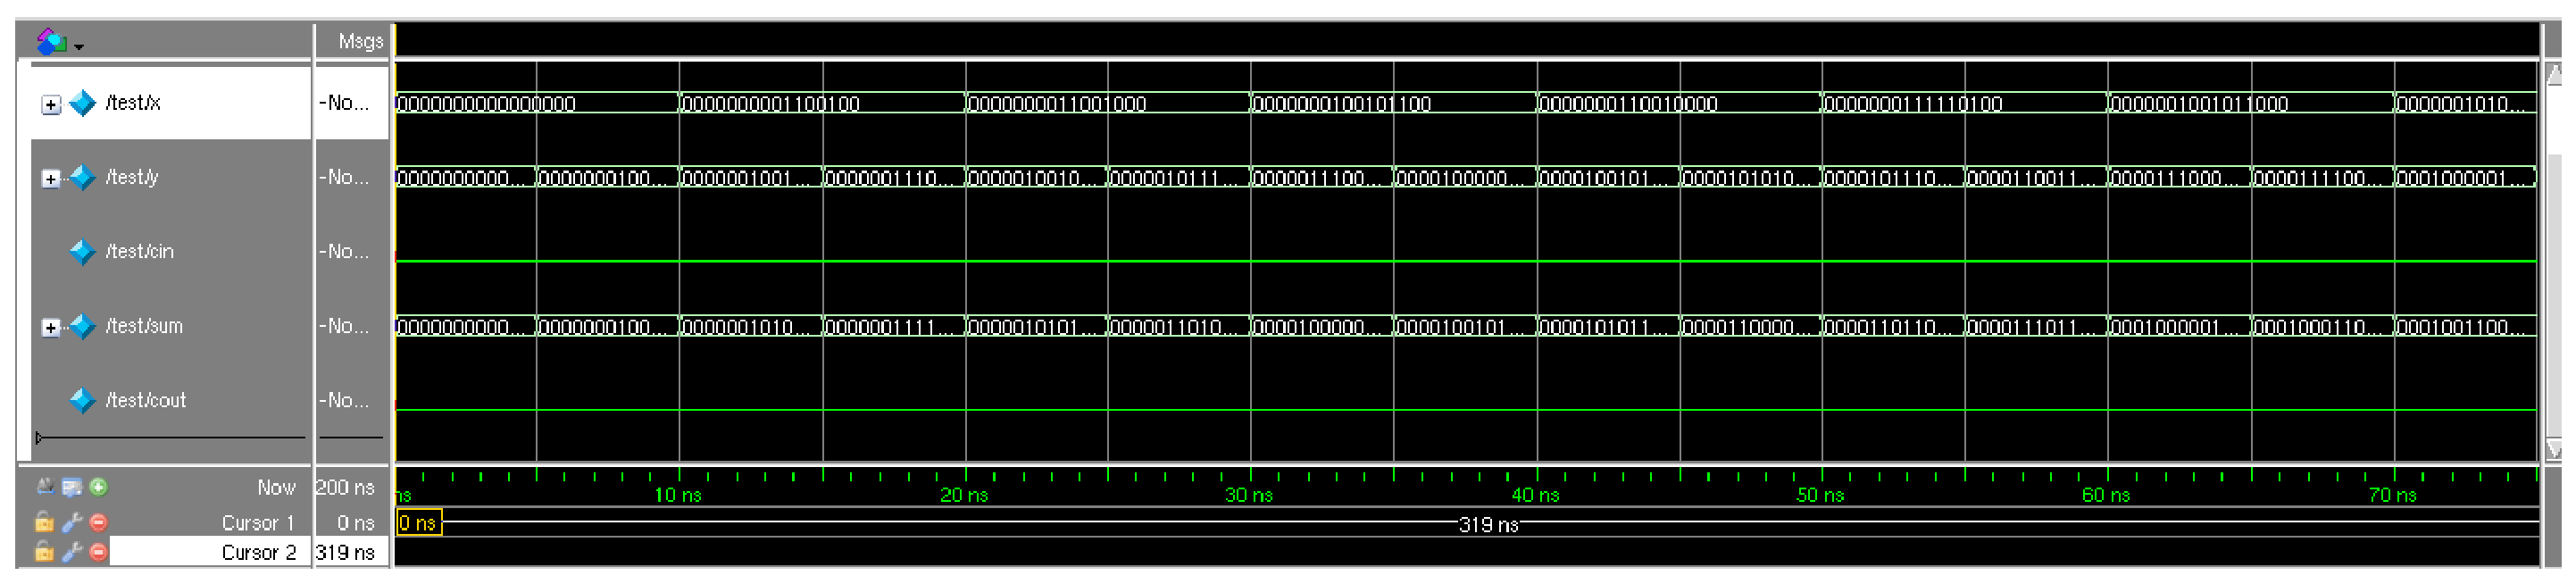
\includegraphics[width=13cm]{images/fig06.eps}
    \caption{機能レベルシミュレーションを行った結果の波形}
    \label{fig:06}
  \end{center}
\end{figure}

しかし、01の2進数表示だったため加算がわかりづらかったので、Radix > Decimalに変更すると、\ref{fig:06-1}の波形が得られた。

\begin{figure}[htb]
  \begin{center}
    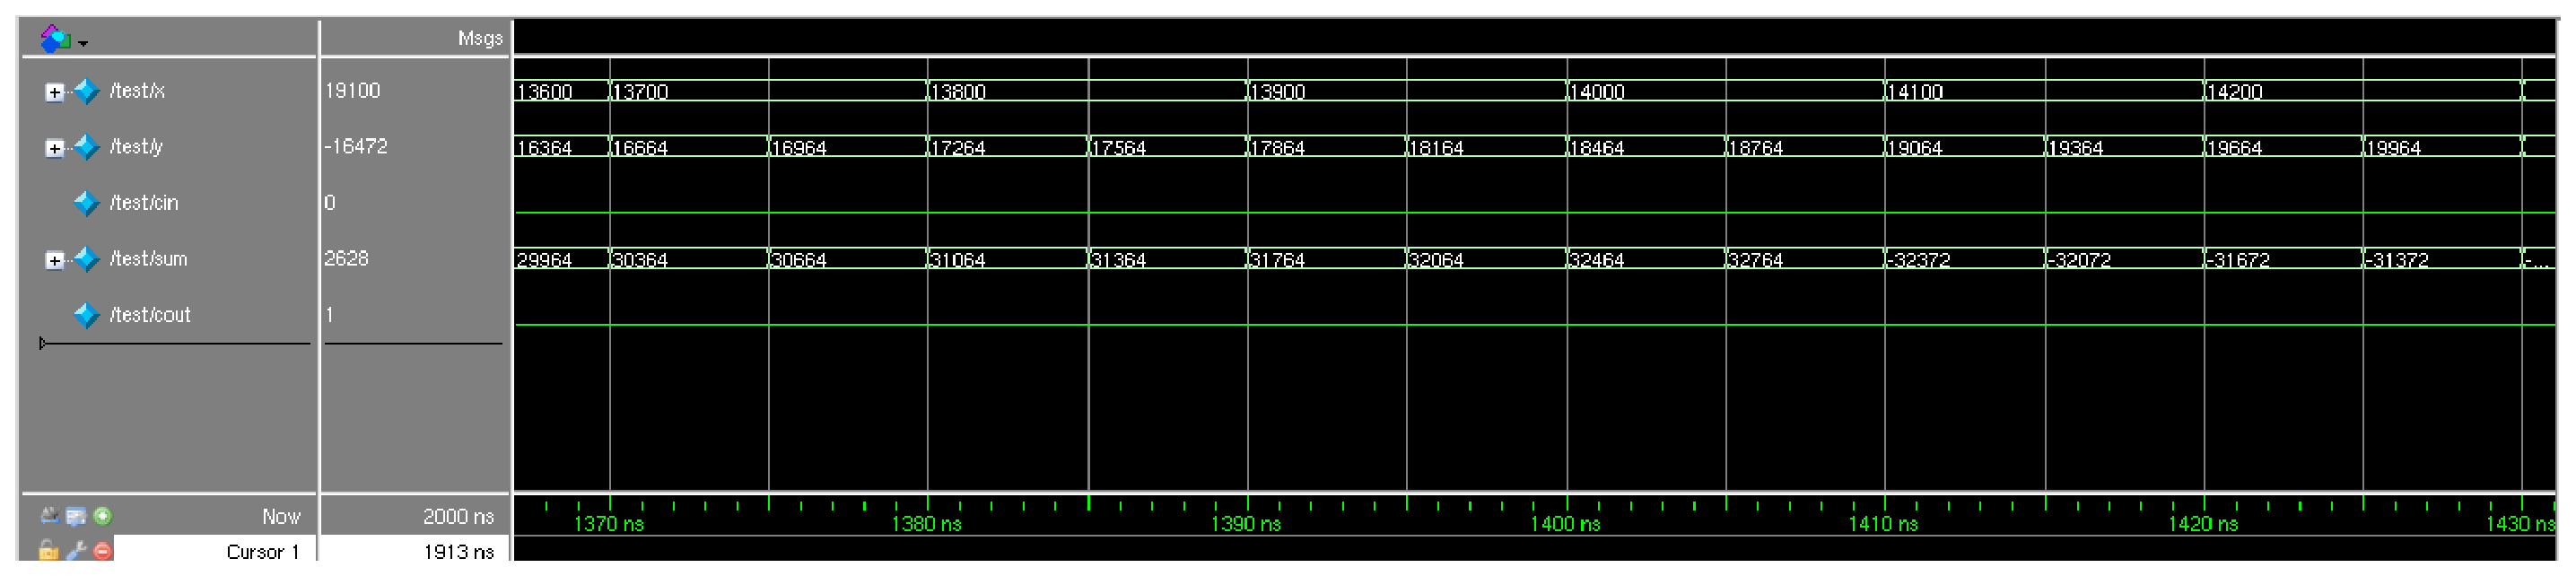
\includegraphics[width=13cm]{images/fig06-1.eps}
    \caption{機能レベルシミュレーションを行った結果の波形}
    \label{fig:06-1}
  \end{center}
\end{figure}

%----------------------------------
\subsubsection{論理合成}
%----------------------------------

コンパイル結果のロジックエレメント数は図\ref{fig:07}のようだった。
ロジックエレメント数は\ref{fig:07}のTotal Logic Elementの部分である。  

\begin{figure}[htb]
  \begin{center}
    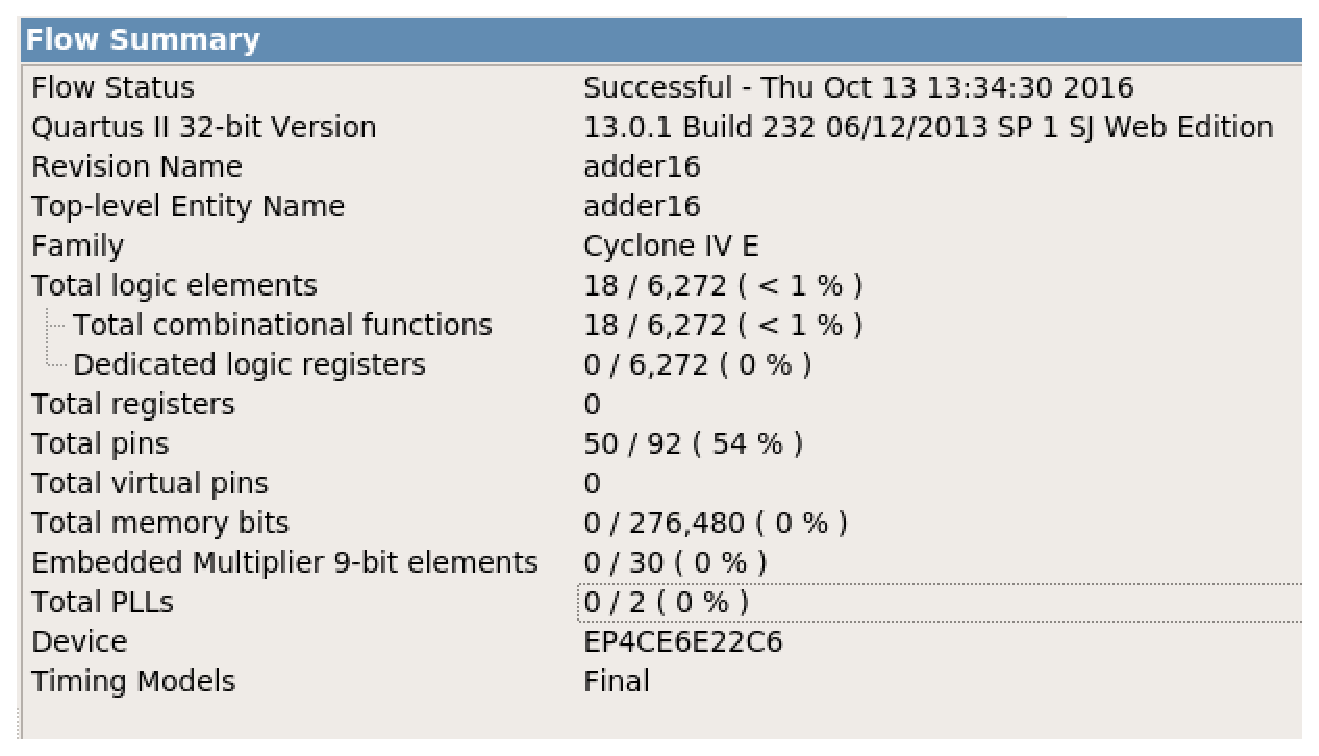
\includegraphics[width=10cm]{images/fig07.eps}
    \caption{ロジックエレメント数}
    \label{fig:07}
  \end{center}
\end{figure}

回路の遅延時間は図\ref{fig:08}の通りだった。
トータルの遅延時間はここでは、11.465nsとなる。

\begin{figure}[htb]
  \begin{center}
    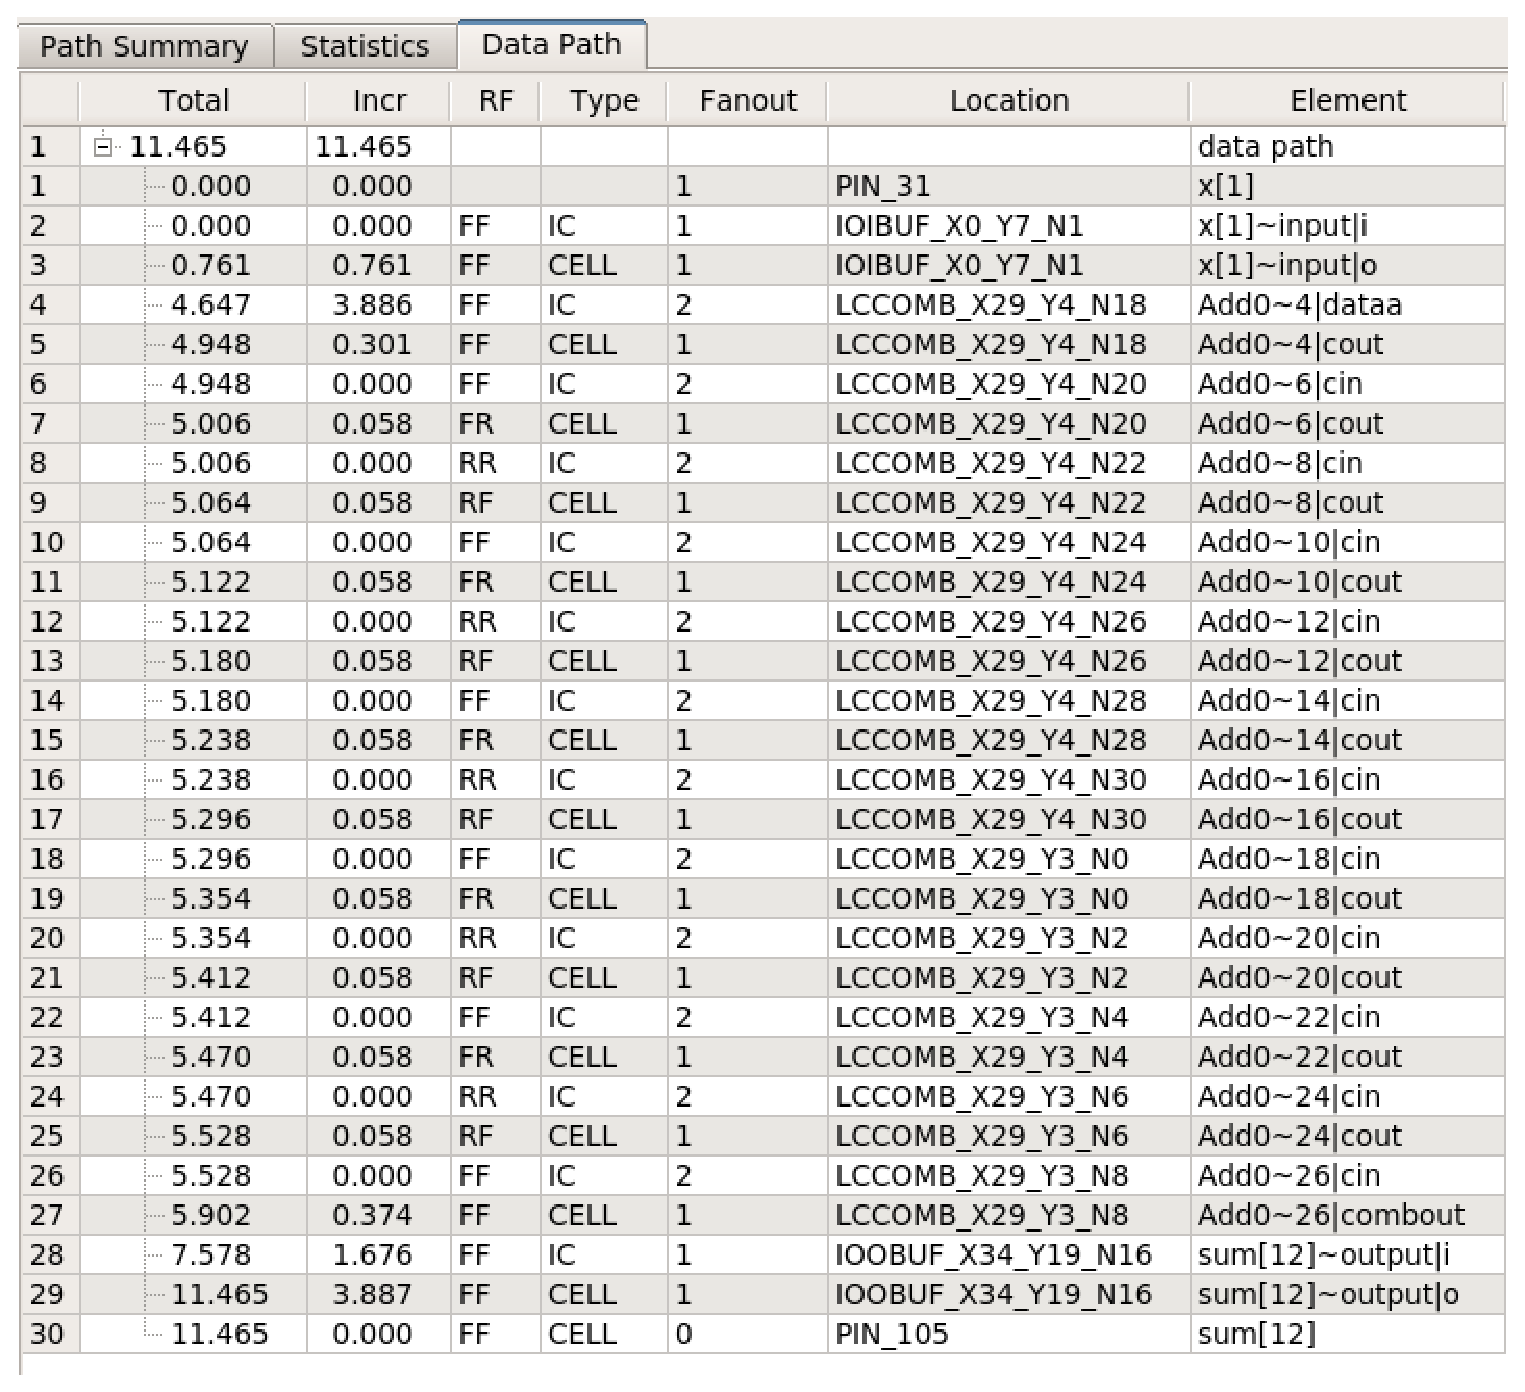
\includegraphics[width=10cm]{images/fig08.eps}
    \caption{遅延時間}
    \label{fig:08}
  \end{center}
\end{figure}

実験結果の回路は図\ref{fig:09}の通りだった。

\begin{figure}[htb]
  \begin{center}
    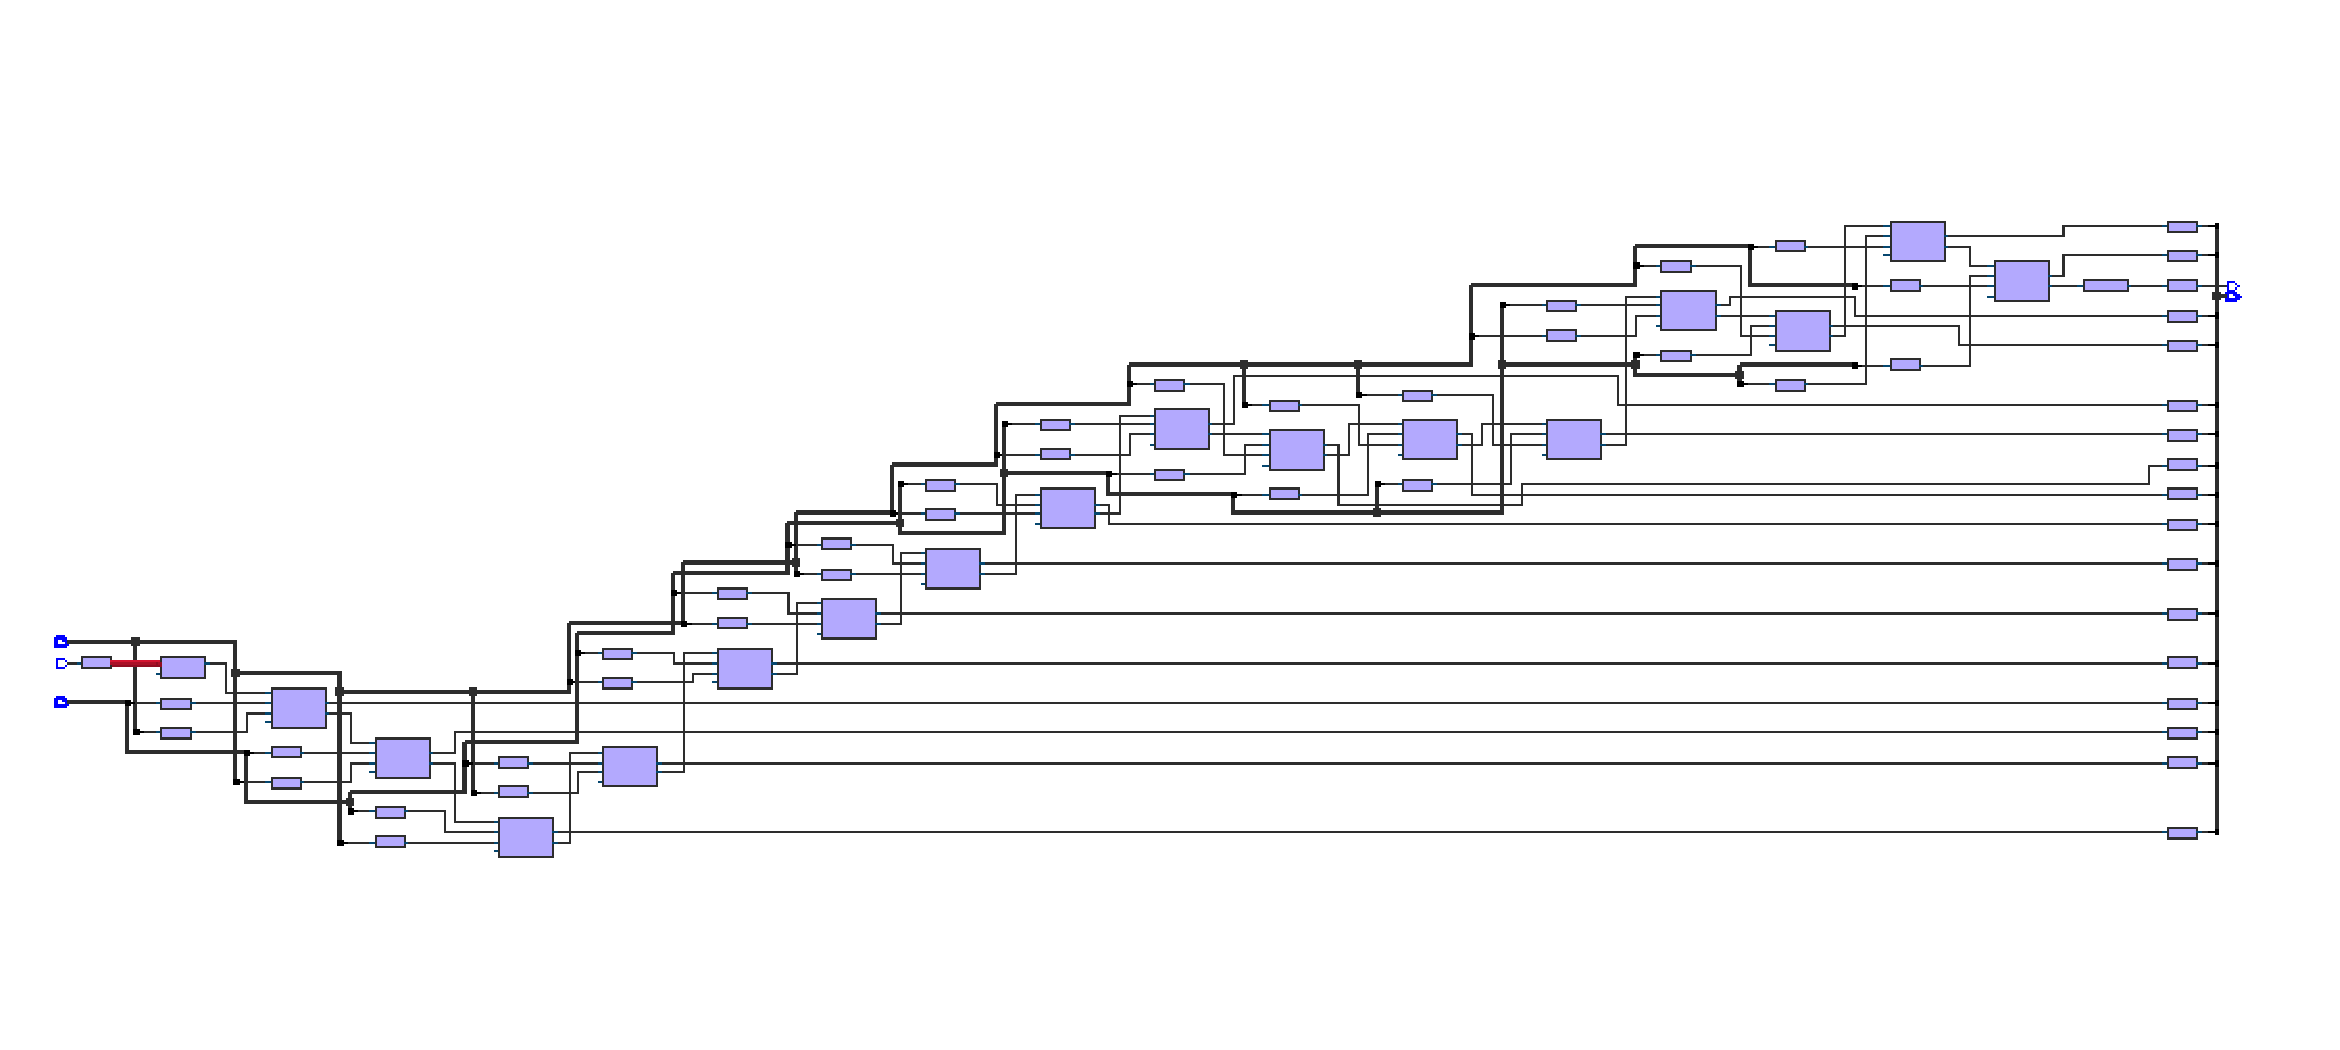
\includegraphics[width=13cm]{images/fig09.eps}
    \caption{16ビット加算回路}
    \label{fig:09}
  \end{center}
\end{figure}


%---------------------------------------------------------------------
\subsection{考察}
%---------------------------------------------------------------------

%----------------------------------
\subsubsection{機能レベルシミュレーション結果に対する評価}
%----------------------------------

図\ref{fig:06-1}から、期待通りに加算が行われている事が分かる。
ある時間軸上の{\tt sum}の値が、同じ時間軸上にある{\tt x, y}の和になっていることが確認できた。

{\tt sum}は16ビット長で、今2進数をDecimal型で表現しているので、$32,768 ~ 32,767$までしか表現ができない。この事も
図\ref{fig:06-1}の後半で符号が反転してあふれている事から確認できた。

%----------------------------------
\subsubsection{回路構成とロジックエレメント数の関係の検討}
%----------------------------------

図\ref{fig:09}の回路構成は膨大で、その仕組みを検討することが困難なので、まずは一般的な4ビット加算器が論理回路を確認することにする。
図\ref{fig:10}のように、桁上げ入力{\tt Ci}と入力{\tt A, B}が各全加算器(Full Adder: FA)に入力されている。
一方、各FAからは、出力値{\tt Si}と桁上げ出力{\tt Ci}が出力されている。
{\tt Si}が加算の結果となる。

\begin{figure}[htb]
  \begin{center}
    \includegraphics[width=6cm]{images/fig10ps}
    \caption{4ビット加算機の論理回路図(文献\cite{hdl}を参考に作成)}
    \label{fig:10}
  \end{center}
\end{figure}

この4ビット加算器の回路と16ビット加算器についても、同様の仕組みである。
図\ref{fig:09}にも4ビット加算器で示した、全加算器の入力と桁上げ入力の2入力が右側のFAにつながっていて、そのFAから
計算結果と桁上げ入力が出力されて、それがまた右側のFAにつながっていることが推測できる。

16ビットの加算器において、FAがロジックエレメントの際章単位であると推察できる。
しかし、ロジックエレメント数が実験結果より18であると示されていた。これは、{\tt cin, cout}と全加算器の間にある、
空のブロックがこのロジックエレメントに含まれていると仮説を立てると、示された数と合う。
2~15坂めのFAの桁上げ入出力によって繋がれている前後がロジックエレメントであるので、1, 16坂めも同様にロジックエレメントに接続
されていると推測した。
しかし、空のロジックエレメントが生じた原因は分からなかった。

\clearpage

%===================================================================
\section{16ビット加算をする順序回路の設計(実験3)}
%===================================================================

%---------------------------------------------------------------------
\subsection{目的・概要}
%---------------------------------------------------------------------

今回の実験では、16ビット加算回路を順序回路で設計する。

順序回路は、出力が過去の入力にも依存する論理回路で、その回路は実験2で構成したような
組み合わせ回路部分と記憶回路部分によって表現される。
記憶回路部分は組み合わせ回路からの出力を一時的に記憶して、その記憶された状態が次回の組み合わせ回路部分の入力となる。
今回の実験では記憶回路(フリップフロップ)をクロック入力のエッジによってイベントに同期させて動作させる。
また、このように回路全体が一つのクロックシグナルのイベントによって動作する順序回路を単相クロック同期式順序回路という。
ここでは、この単相クロック同期式順序回路を設計する。

%---------------------------------------------------------------------
\subsection{実験手順}
%---------------------------------------------------------------------

今回の実験は、実験2とと同じ16ビット加算器を順序回路での設計を行った。
仕様は以下の通りである。

\begin{itemize}
  \item 入力: 被演算数x, y(16ビット), 桁上げ入力cin(1ビット)
  \item 出力: 和sum(16ビット), 桁上げ出力cout(1ビット)
  \item 機能: x+y を計算して、和と桁上げを出力する組み合わせ回路
\end{itemize}

はじめに、Verilog HDLで順序回路記述した。そのコードは以下の通りである。

\lstinputlisting[caption=16ビット加算順序回路,label=adder16s.v]{../../jikken3/adder16s.v}

このコードの構造を説明する。

\begin{itemize}
  \item 1~4行目はコメントである。
  \item 6行目で今回のモジュールを定義した。ここでの引数は実験2のそれとは異なり、入力として{\tt clk, reset}が増えている。
  \item 7~10行目では入力用16ビットのx, yと1ビットのclk, reset, cin。
          そして、出力用に16ビットのsum, 1ビットのcoutとなっている。
  \item 12行目で現在の値を記憶しておくフリップフロップ(16ビットレジスタ){\tt r0, r1}を宣言した。
  \item 14行目で出力ポートへの代入を行った。
  \item 16行目以降で処理を記述した。
	  {\tt always}が発生する条件として、クロックの立ち上がり{\tt posedge clk(positive edge clk)}とリセット信号の立ち下がり{\tt negedge reset(negative edge reset)}を検出している。
  \item 17,18行目で {\tt reset == 1'b0}、 つまり、{\tt reset}バイナリが0であるとき、{\tt r0, r1}をリセットする制御を記述した。
	  また、{\tt <=}とかかれる代入は、ノンブロッキング代入と呼ばれ、{\tt begin ~ end}内の右辺の評価が全て行われた後に、全ての代入が同時に実行される。
  \item 19, 20行目で {\tt reset != 1'b0}、つまり、{\tt reset}バイナリが1のときは{\tt r0}に{\tt x}の値を、{\tt r1}に{\tt y}の値を代入する制御を記述した。
\end{itemize}

次に、上記の順序回路のテストベンチを作成した。そのコードは以下の通り。

\lstinputlisting[caption=16ビット加算順序回路のテストベンチ,label=test_adder16s.v]{../../jikken3/test_adder16s.v}

同様にこのコードの構造を説明する。

\begin{itemize}
  \item 1~4行目はコメントである。
  \item 6, 7行目で今までの実験同様、テストの単位時間の設定と今回の回路の取り込みを行っている。
  \item 8行目以降で、{\tt test}モジュールを宣言している。
  \item 10, 11行目で信号を与える入力ポートを宣言した。
  \item 13, 14行目で信号を観測する対象のポートを宣言した。
  \item 16行目で16ビット加算器の実体化を行った。
  \item 18~21行目でクリック信号を出力するように記述した。5nsごとに{\tt clk}はビット反転する。
  \item 22~25行目で演算の対象となるx, yにそれぞれ100, 200を加算する処理を記述した。ここでしっかり加算されているかは
          実験結果の波形を見れば確かめられる。8nsごとにこ処理は実行される。
  \item 27~31行目は初期値の設定を行った。
           29, 30行目はリセット信号の挙動を確かめるために処理開始後20nsまでは{\tt 1}にその後20ns後に{\tt 0}になったのち、また戻る処理を記述した。
\end{itemize}

次に,機能レベルシミュレーション,論理合成を行った.
実験の手続きは,実験1と同様なので省略する.

%---------------------------------------------------------------------
\subsection{実験結果}
%---------------------------------------------------------------------

%----------------------------------
\subsubsection{機能レベルシミュレーション}
%----------------------------------

図\ref{fig:11}に示す波形を得た。

\begin{figure}[htb]
  \begin{center}
    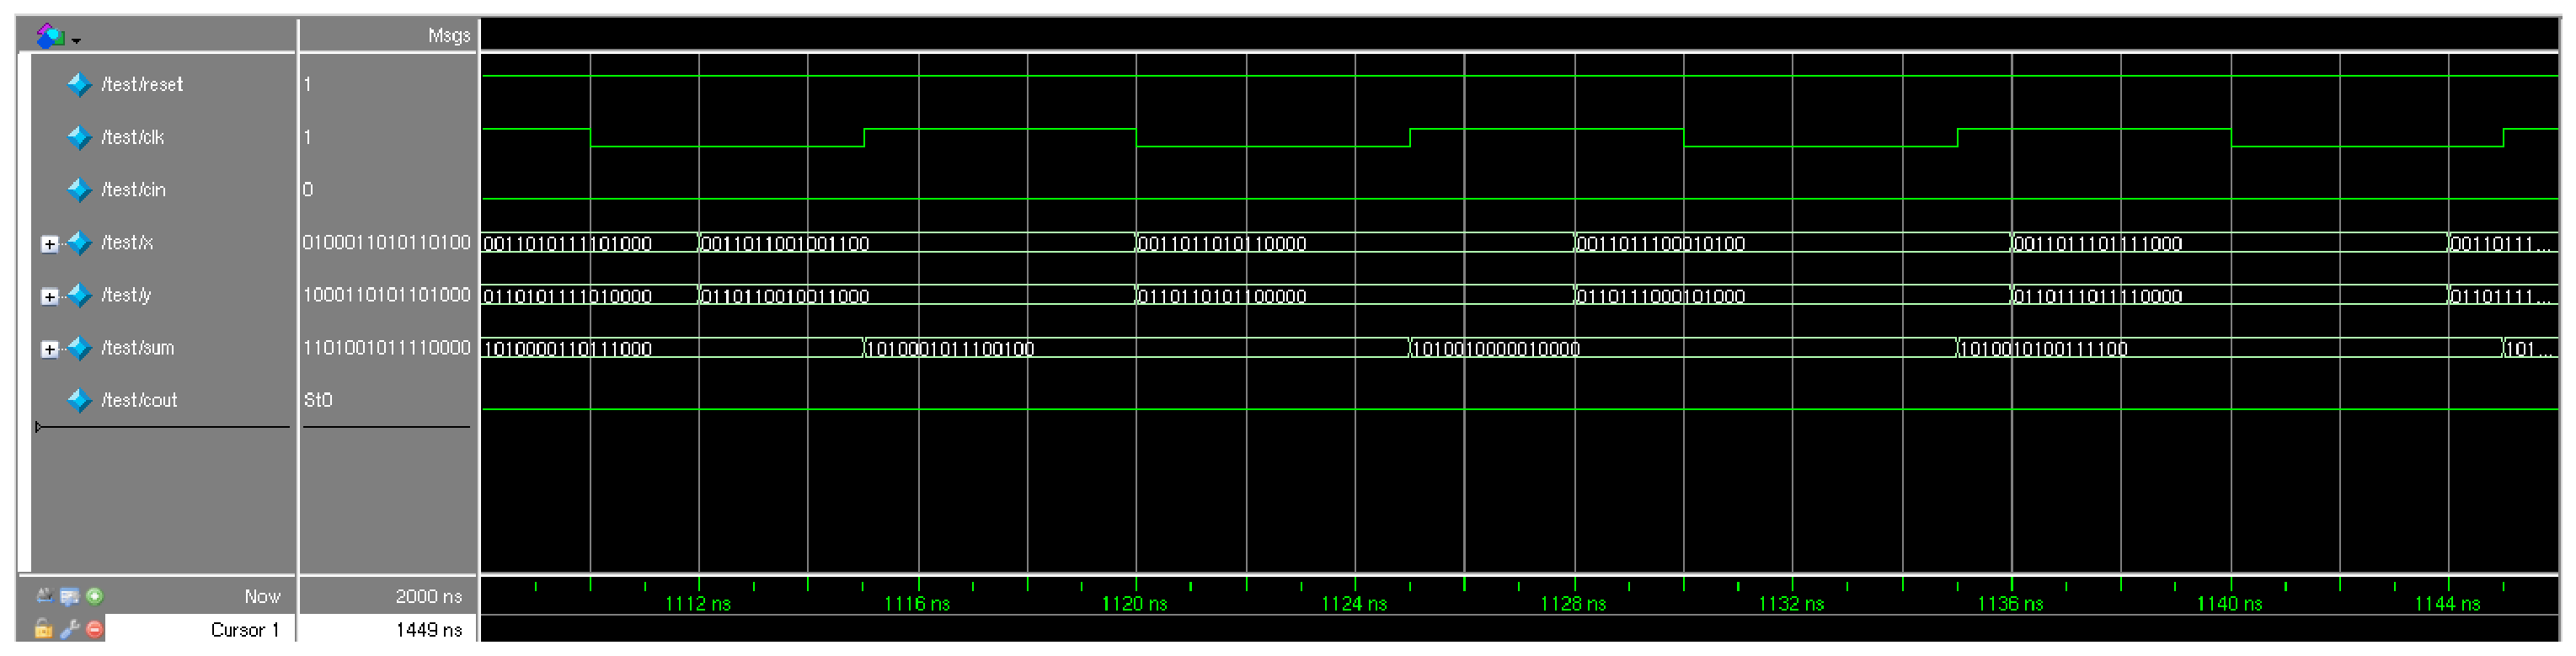
\includegraphics[width=13cm]{images/fig11.eps}
    \caption{機能レベルシミュレーションを行った結果の波形}
    \label{fig:11}
  \end{center}
\end{figure}

実験2と同様に01の2進数表示だったため加算がわかりづらかったので、Radix > Decimalに変更すると、\ref{fig:11-1}の波形が得られた。

\begin{figure}[htb]
  \begin{center}
    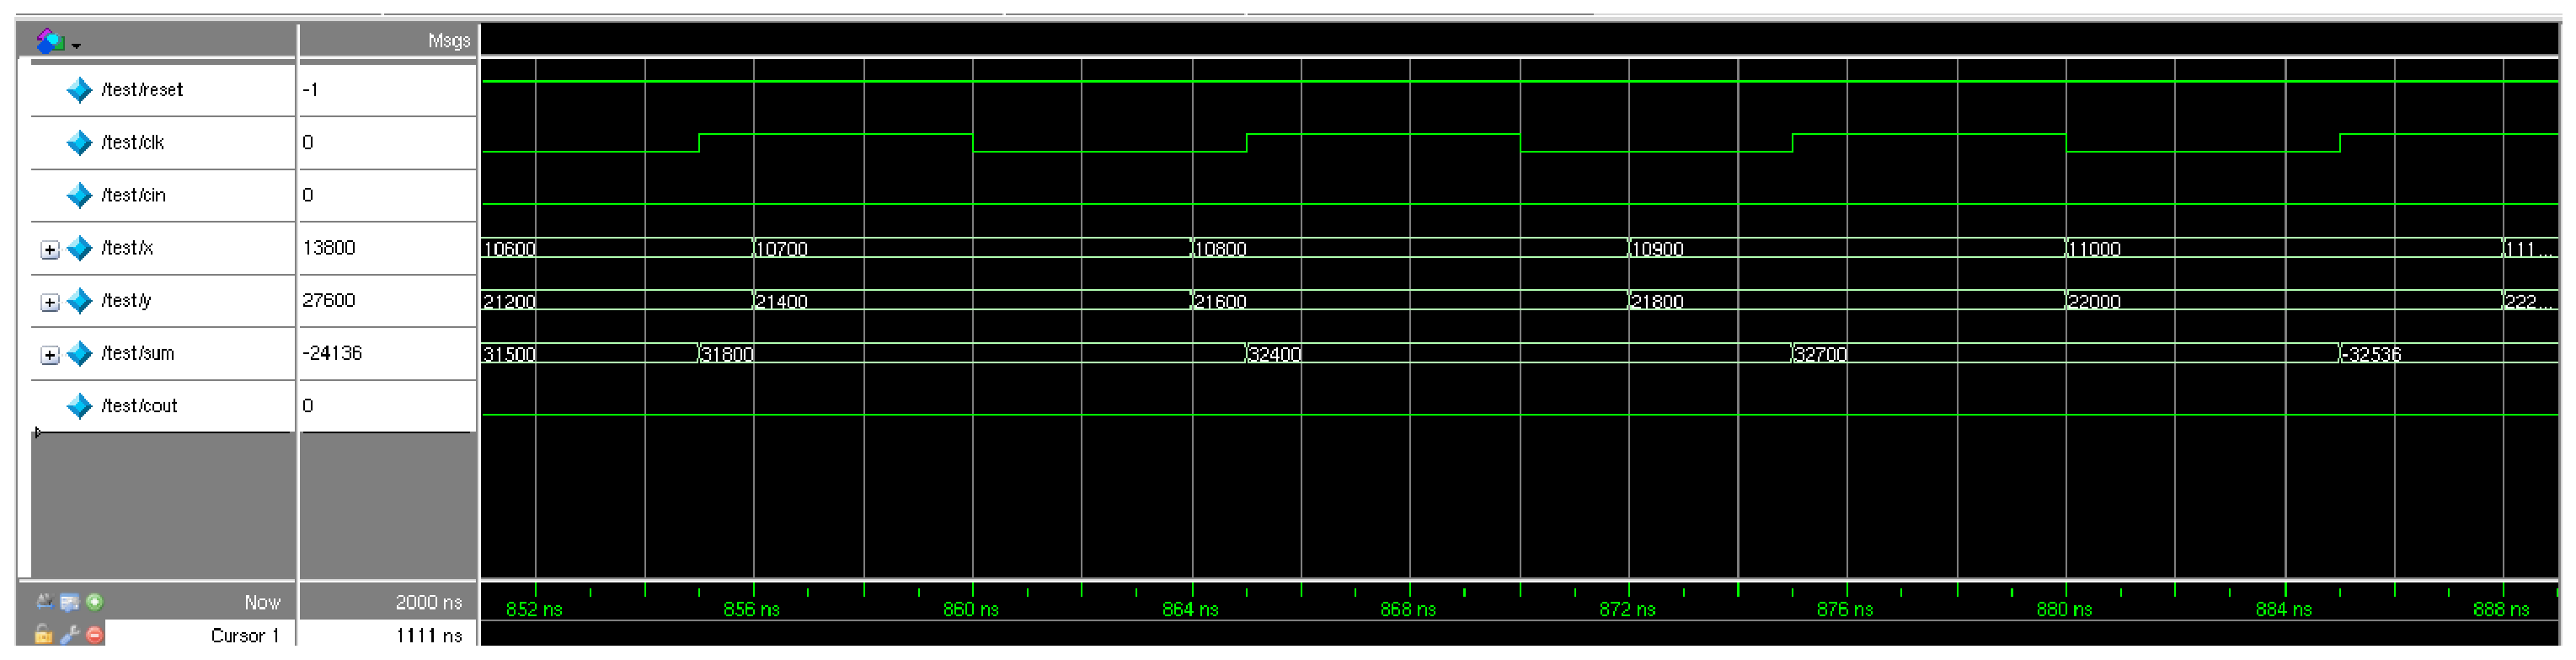
\includegraphics[width=13cm]{images/fig11-1.eps}
    \caption{機能レベルシミュレーションを行った結果の波形}
    \label{fig:11-1}
  \end{center}
\end{figure}

%----------------------------------
\subsubsection{論理合成}
%----------------------------------

コンパイル結果のロジックエレメント数は図\ref{fig:12}のようだった。
ロジックエレメント数は\ref{fig:12}のTotal Logic Elementの部分である。  

\begin{figure}[htb]
  \begin{center}
    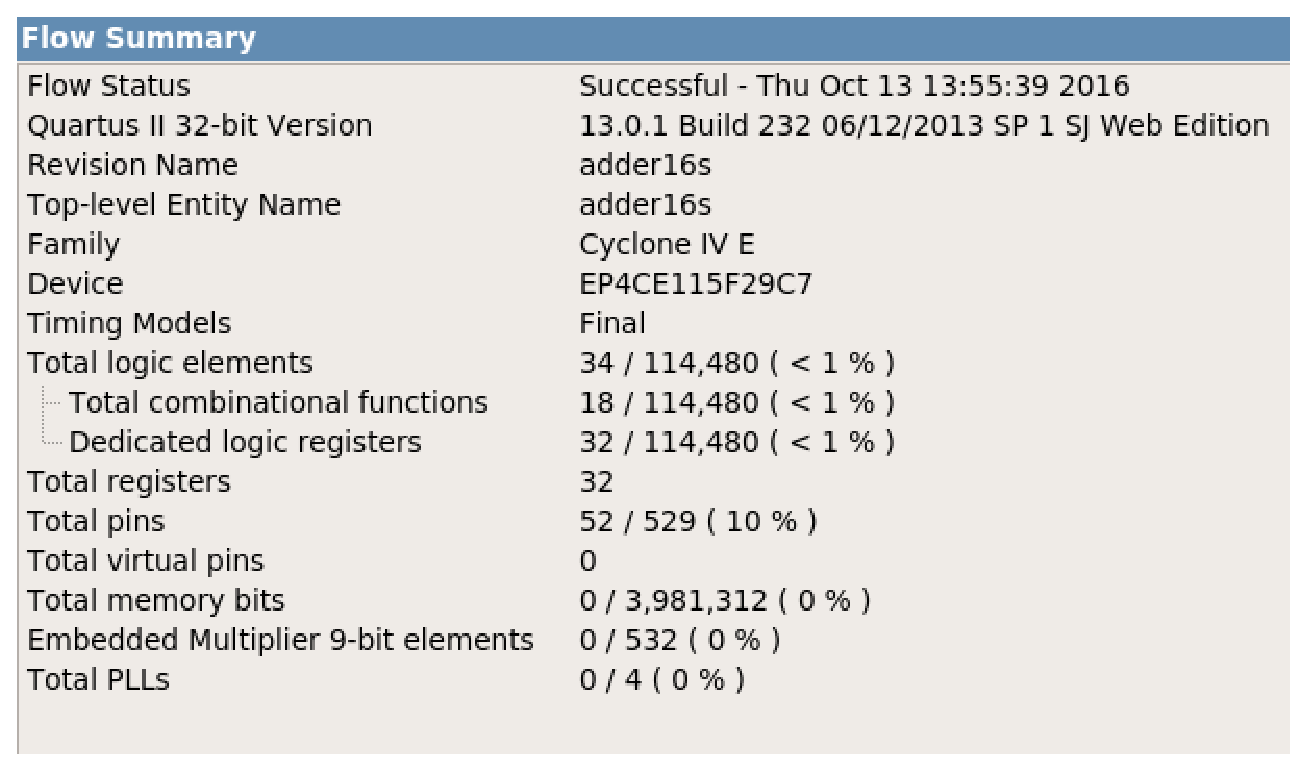
\includegraphics[width=13cm]{images/fig12.eps}
    \caption{ロジックエレメント数}
    \label{fig:12}
  \end{center}
\end{figure}

回路の遅延時間は図\ref{fig:13}の通りだった。
トータルの遅延時間はここでは、10.218nsとなる。

\begin{figure}[htb]
  \begin{center}
    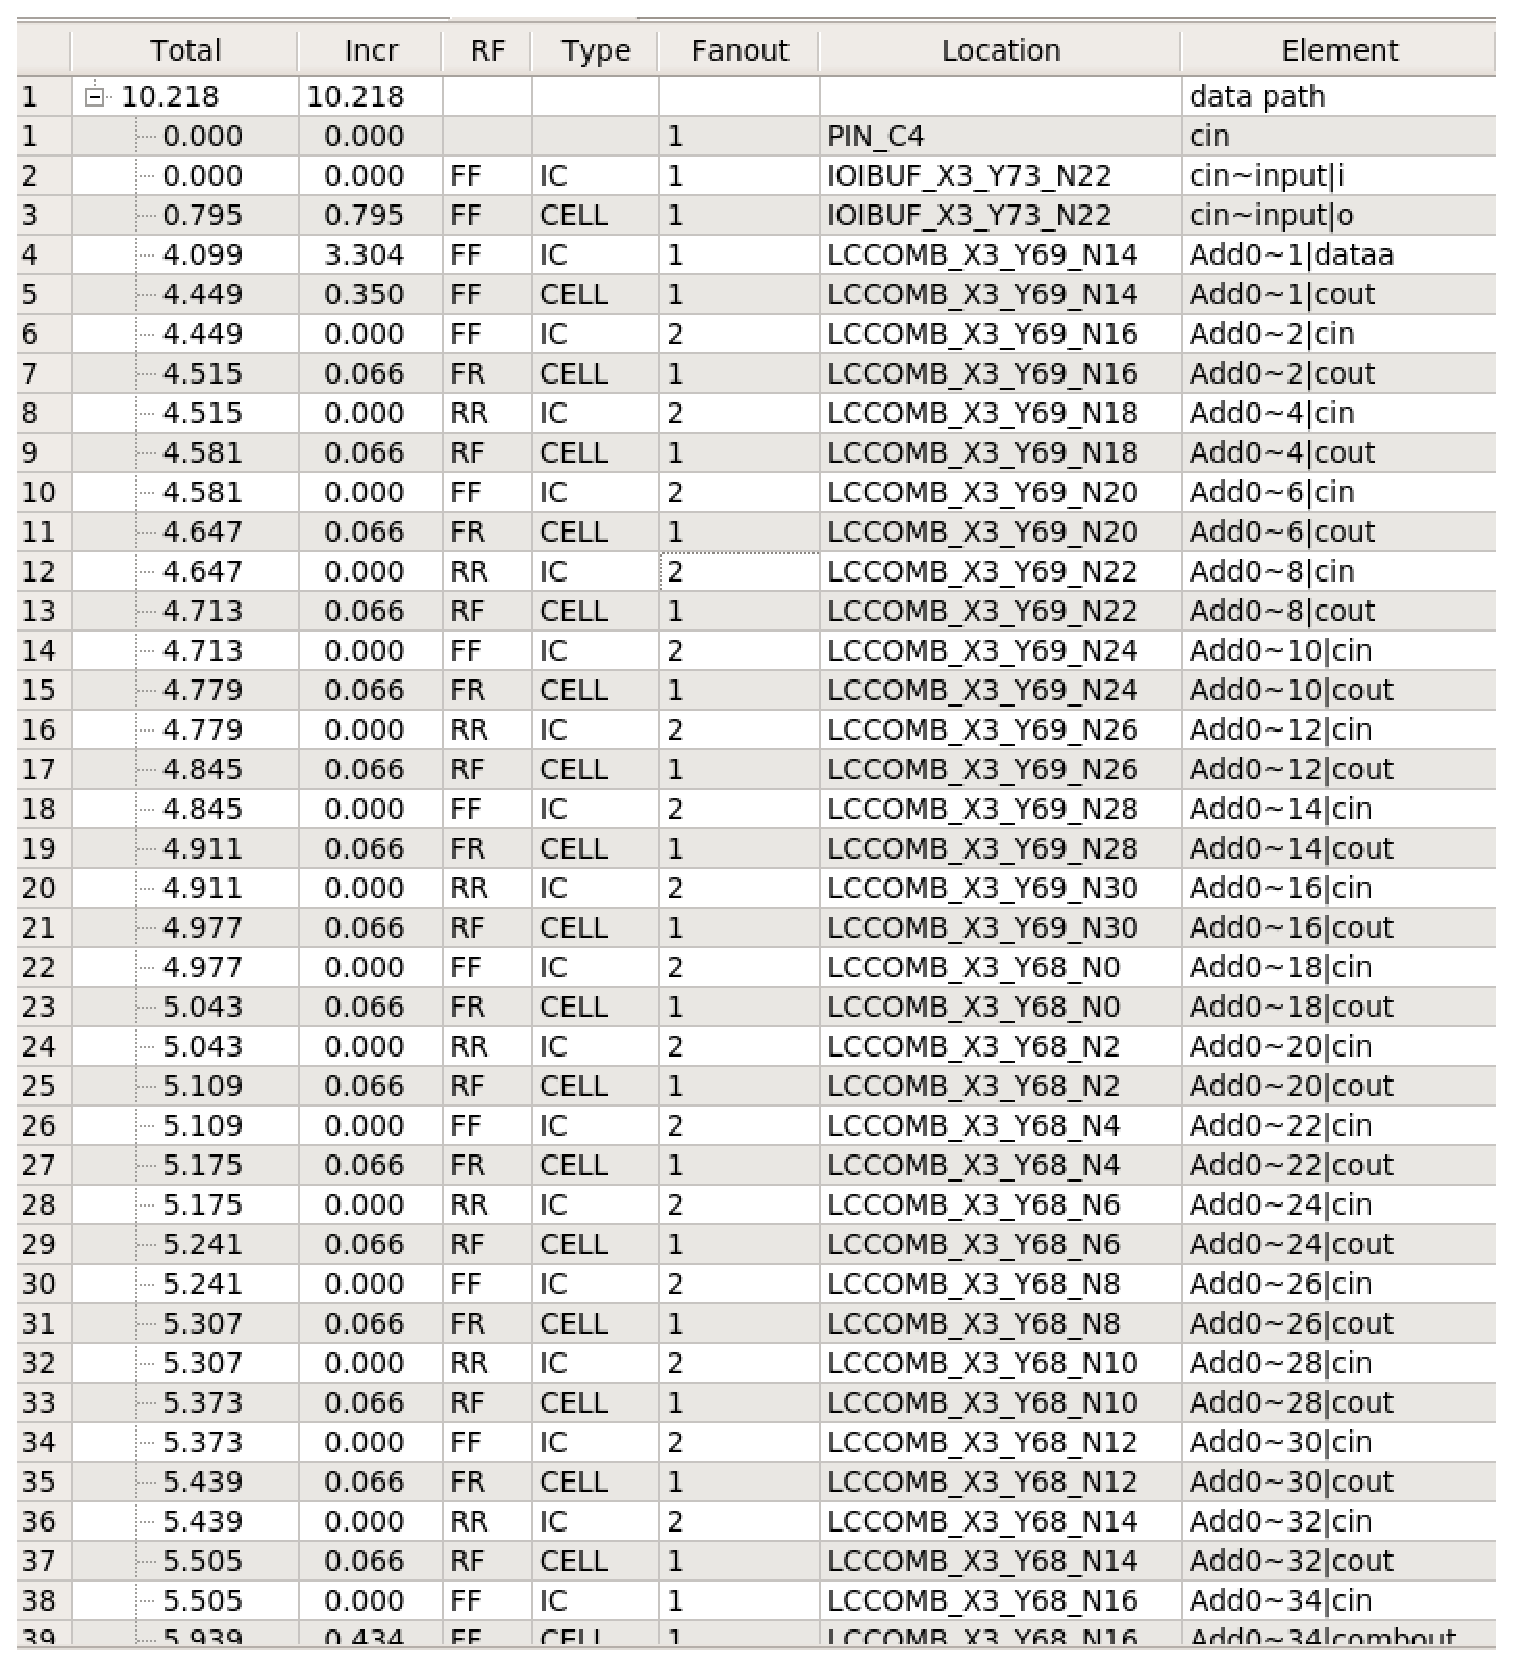
\includegraphics[width=13cm]{images/fig13.eps}
    \caption{遅延時間}
    \label{fig:13}
  \end{center}
\end{figure}

最適化後の回路は図\ref{fig:14}の通りだった。

\begin{figure}[htb]
  \begin{center}
    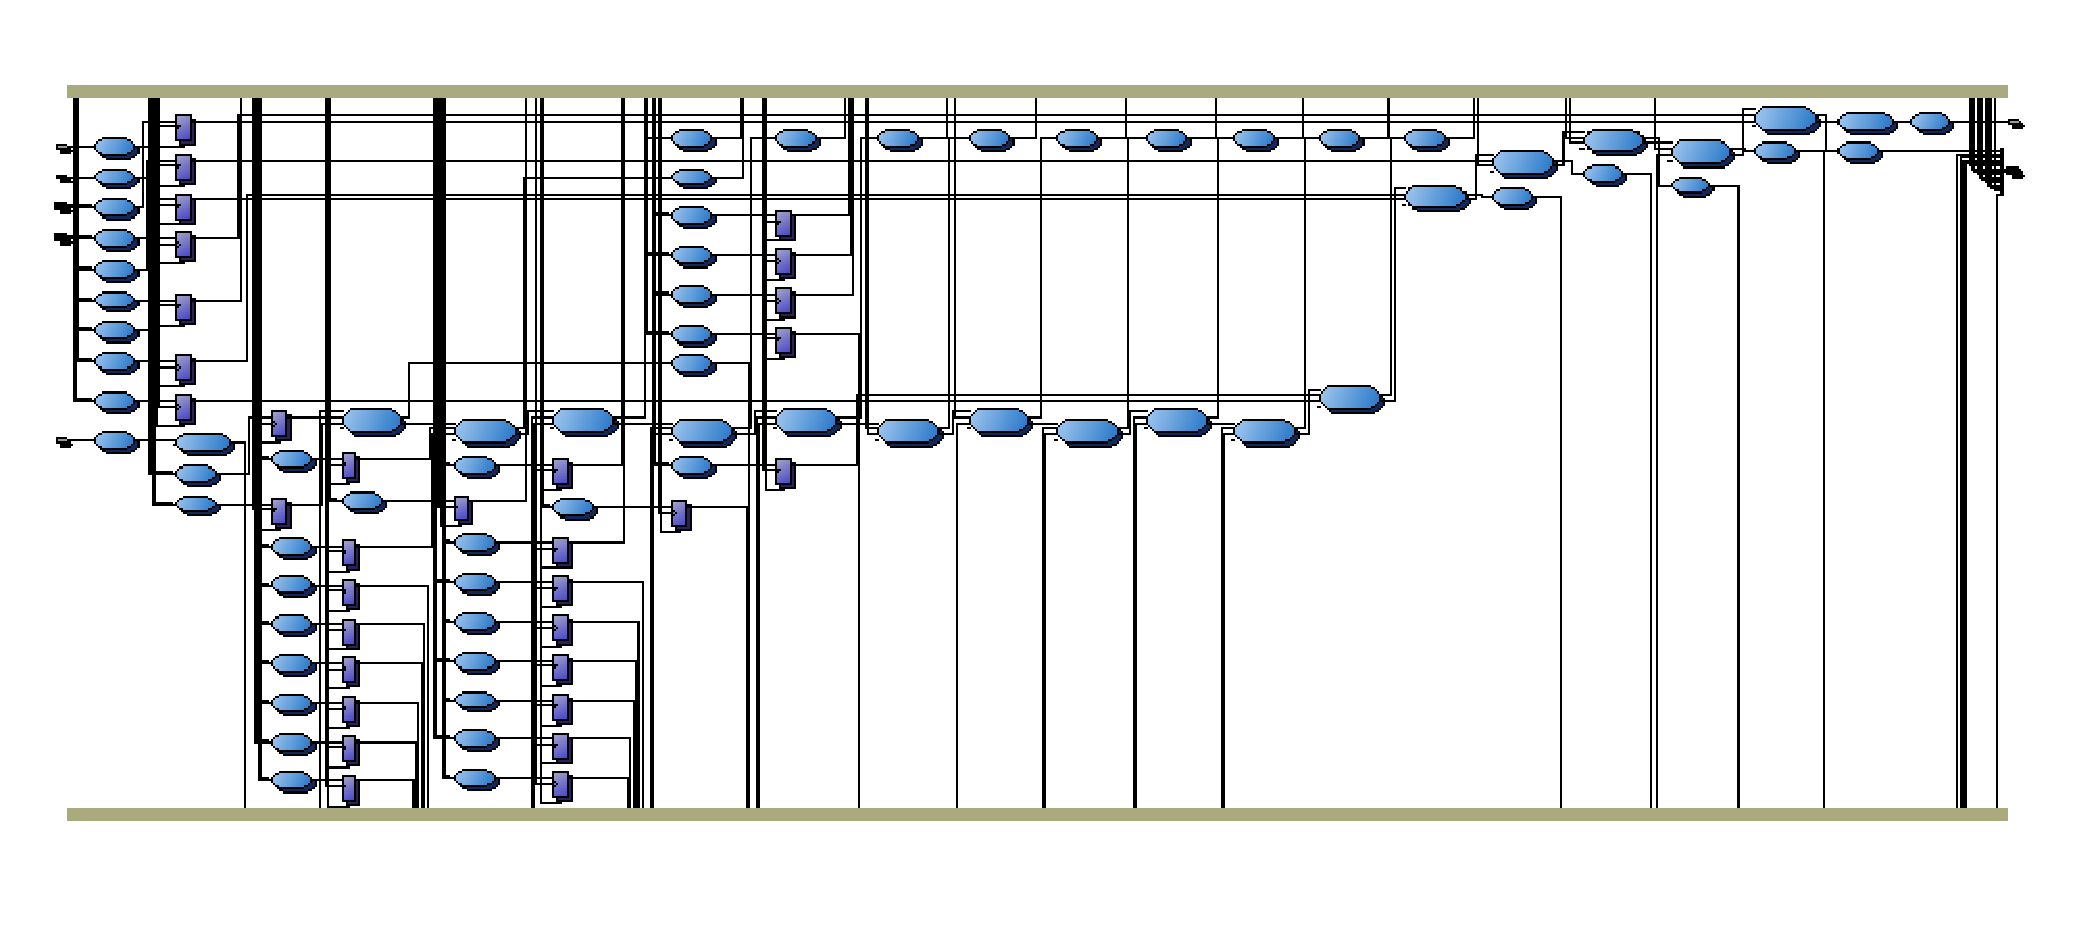
\includegraphics[width=13cm]{images/fig14.eps}
    \caption{16ビット加算順序回路}
    \label{fig:14}
  \end{center}
\end{figure}

%---------------------------------------------------------------------
\subsection{考察}
%---------------------------------------------------------------------

実験2と同じ16ビット加算回路を今回の実験では組み合わせ回路ではなく、順序回路で構成した。

論理合成の結果をみてみると、入力のみから出力が決まる組み合わせ回路に比べて、前の出力の情報を
記録しておくためにレジスタが必要になったため、ロジックエレメント数は結果的に実験2に比べて大きくなっていた。
しかし、遅延時間は組み合わせ回路の加算回路に比べて、減少していたため、これは順序回路を用いた結果回路が小さくなった
ことだと推測される。順序回路を設計することで、テストしなければいけないことが増えたり、設計にバグが混入しやすくしたり
とメリットとデメリットを含むので状況に応じて使い分けをするのが、適切な方法だと思われる。


\clearpage

%===================================================================
\section{1桁BCDカウンタの設計(実験課題1)}
%===================================================================

%---------------------------------------------------------------------
\subsection{目的・概要}
%---------------------------------------------------------------------

今回の実験では、1桁BCDカウンタを設計する。
この順序回路をVerilog HDLで記述して、機能レベルシミュレーションにより動作を確認、
また、論理合成を実行して合成結果を確認する。

%---------------------------------------------------------------------
\subsection{実験手順}
%---------------------------------------------------------------------

今回の実験は、1桁のBCDカウンタの設計を行った。
仕様は以下の通りである。

\begin{itemize}
  \item 入力: クロックclk(1ビット), リセットreset(1ビット), カウントアップ信号x(1ビット)
  \item 出力; カウンタ値出力 bcd1_out(4ビット)
  \item 機能: リセットが0になると出力の各ビットは0になる(非同期リセット)。出力値はclkが0から1に変化かつカウントアップ信号が
	   1になるたびにカウントアップして、0000 -> 0001 -> 0010 -> ... -> 1001 -> 0000 -> 0001 -> ...となる。
\end{itemize}

はじめに、Verilog HDLで順序回路記述した。そのコードは以下の通りである。

\lstinputlisting[caption=1桁BCDカウンタ,label=bcd1.v]{../../jikken-kadai1/bcd1.v}

このコードの構造を説明する。

\begin{itemize}
  \item 1~4行目はコメントである。
  \item 6行目から、1桁BCDカウンタのモジュールを記述した。
  \item 7, 8行目で入出力用に宣言。
  \item 10行目にカウントを記憶するための4ビットのレジスタを宣言した。
  \item 12行目で出力{\tt bcd1\_out}にレジスタの値{\tt count\_reg}を代入した。
  \item 15行目から{\tt always}ブロックの記述をした。これは実験3の時の同様で、クロックの立ち上がりとリセット信号の立ち下がりを検出している。
  \item 16行目の条件分岐では{\tt reset}が 0 or 1で振り分けている。
  \item 17 ~ 22行目までは、{\tt reset == 0}の時で、この時は{\tt count\_reg}に0を代入している。ここで、上のコメント文では1ビットずつ0を代入しているが
           一気に0を代入しても、全てのビットが0に置き換わる。
  \item 23~35行目までは{\tt reset == 1}の時の処理。
  \item 25行目では{\tt reset == 1}かつ{\tt x == 1}の時、カウンタをカウントさせる動作をする。
          今回のカウンタは{\tt count\_reg} が {\tt 1001} (10進数では{\tt 9})の時に、レジスタの値を{\tt 0}にする。
          この数値判定はC言語のように{\tt count\_reg == 9}で実現できる。そうでない場合は、{\tt count\_reg}をカウントアップ、つまり1を加算する。
\end{itemize}


続いて、この1桁BCDカウンタを動かすためのテストベンチを作成した。そのコードは以下の通りである。

\lstinputlisting[caption=1桁BCDカウンタのテストベンチ,label=test_bcd1.v]{../../jikken-kadai1/test_bcd1.v}

このコードの構造を説明する。

\begin{itemize}
  \item 1~4行目はコメントである。
  \item 6,7 行目でシミュレーションの単位時間/精度の記述と、今回の回路を取り込んだ。
  \item 9行目から、テストモジュールを宣言する。
  \item 11行目で、入力値を格納するレジスタを宣言した。
  \item 14行目で出力を観測するための信号線{\tt bcd1\_out}を宣言した。
  \item 17行目で{\tt bcd1}を実体化する処理を記述した。
  \item 19~21行目で5nsごとにクリック信号を反転させる記述をした。クリック信号を送っている。
  \item 23~25行目は15nsごとに、{\tt x}をビット反転している。つまり、15nsごとに0と1を行ったり来たりしている。
  \item 27行目からは初期値の設定を行っている。
        {\tt reset}に{\tt 1}を初期化して、20ns後に値を{\tt 0}にした後、またその20ns後に{\tt 1}に戻す処理を記述している。
	  また、このテストベンチはさらにその1000ns後に終了する記述をしている。
\end{itemize}

%---------------------------------------------------------------------
\subsection{実験結果}
%---------------------------------------------------------------------

%----------------------------------
\subsubsection{機能レベルシミュレーション}
%----------------------------------

図\ref{fig:15}に示す波形を得た。

\begin{figure}[htb]
  \begin{center}
    \includegraphics[width=13cm]{images/fig15.eps}
    \caption{機能レベルシミュレーションを行った結果の波形}
    \label{fig:15}
  \end{center}
\end{figure}

%----------------------------------
\subsubsection{論理合成}
%----------------------------------


コンパイル結果のロジックエレメント数は図\ref{fig:16}のようだった。
ロジックエレメント数は\ref{fig:16}のTotal Logic Elementの部分である。  

\begin{figure}[htb]
  \begin{center}
    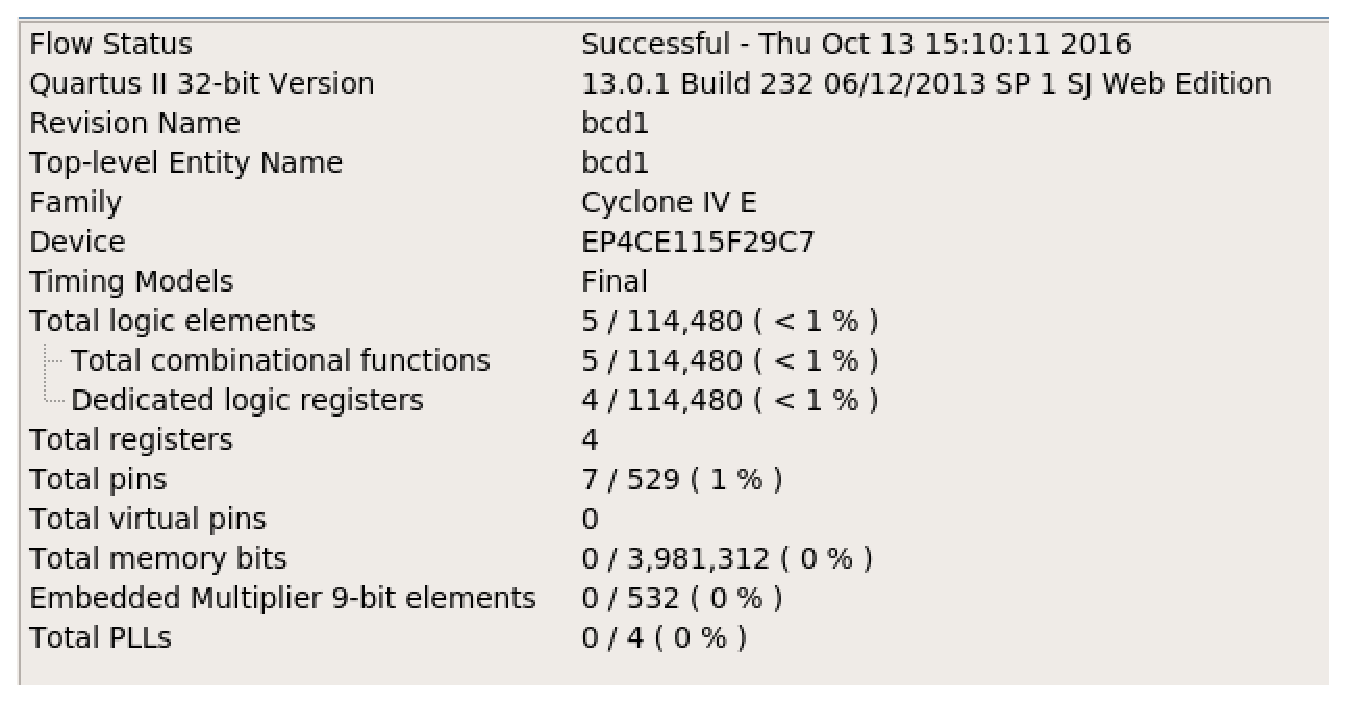
\includegraphics[width=13cm]{images/fig16.eps}
    \caption{ロジックエレメント数}
    \label{fig:16}
  \end{center}
\end{figure}

回路の遅延時間は図\ref{fig:17}の通りだった。
トータルの遅延時間はここでは、5.169nsとなる。

\begin{figure}[htb]
  \begin{center}
    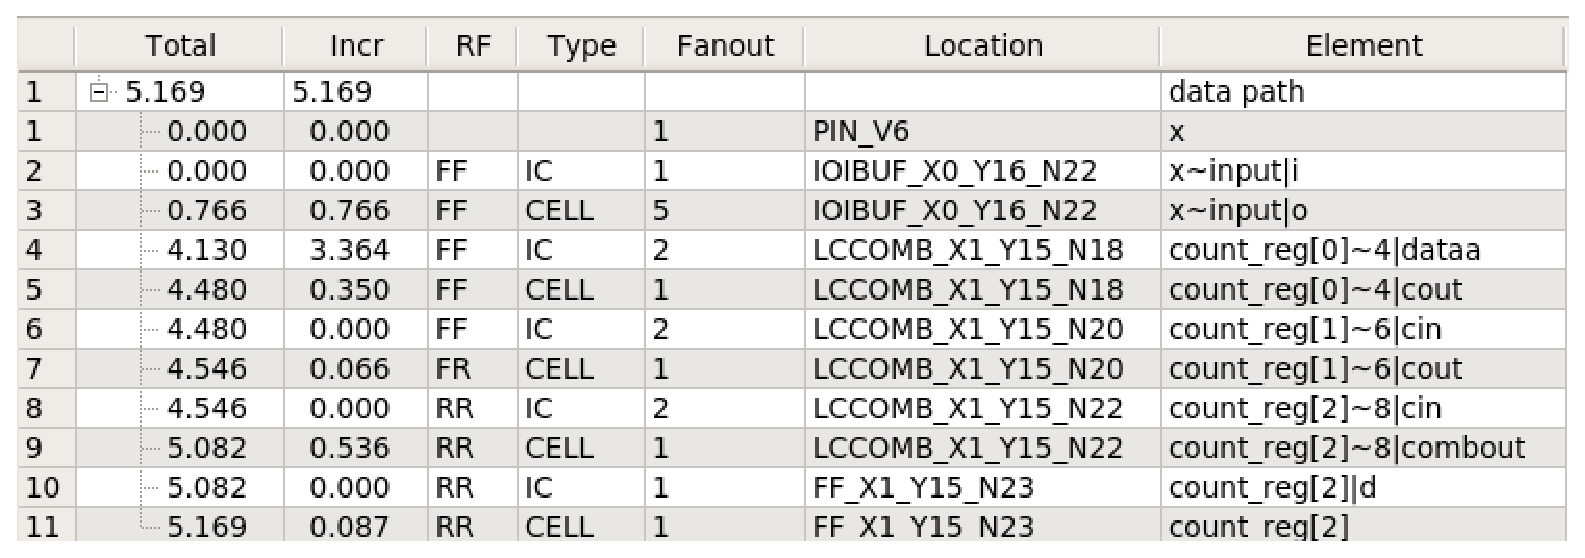
\includegraphics[width=13cm]{images/fig17.eps}
    \caption{遅延時間}
    \label{fig:17}
  \end{center}
\end{figure}

最適化後の回路は図\ref{fig:18}の通りだった。

\begin{figure}[htb]
  \begin{center}
    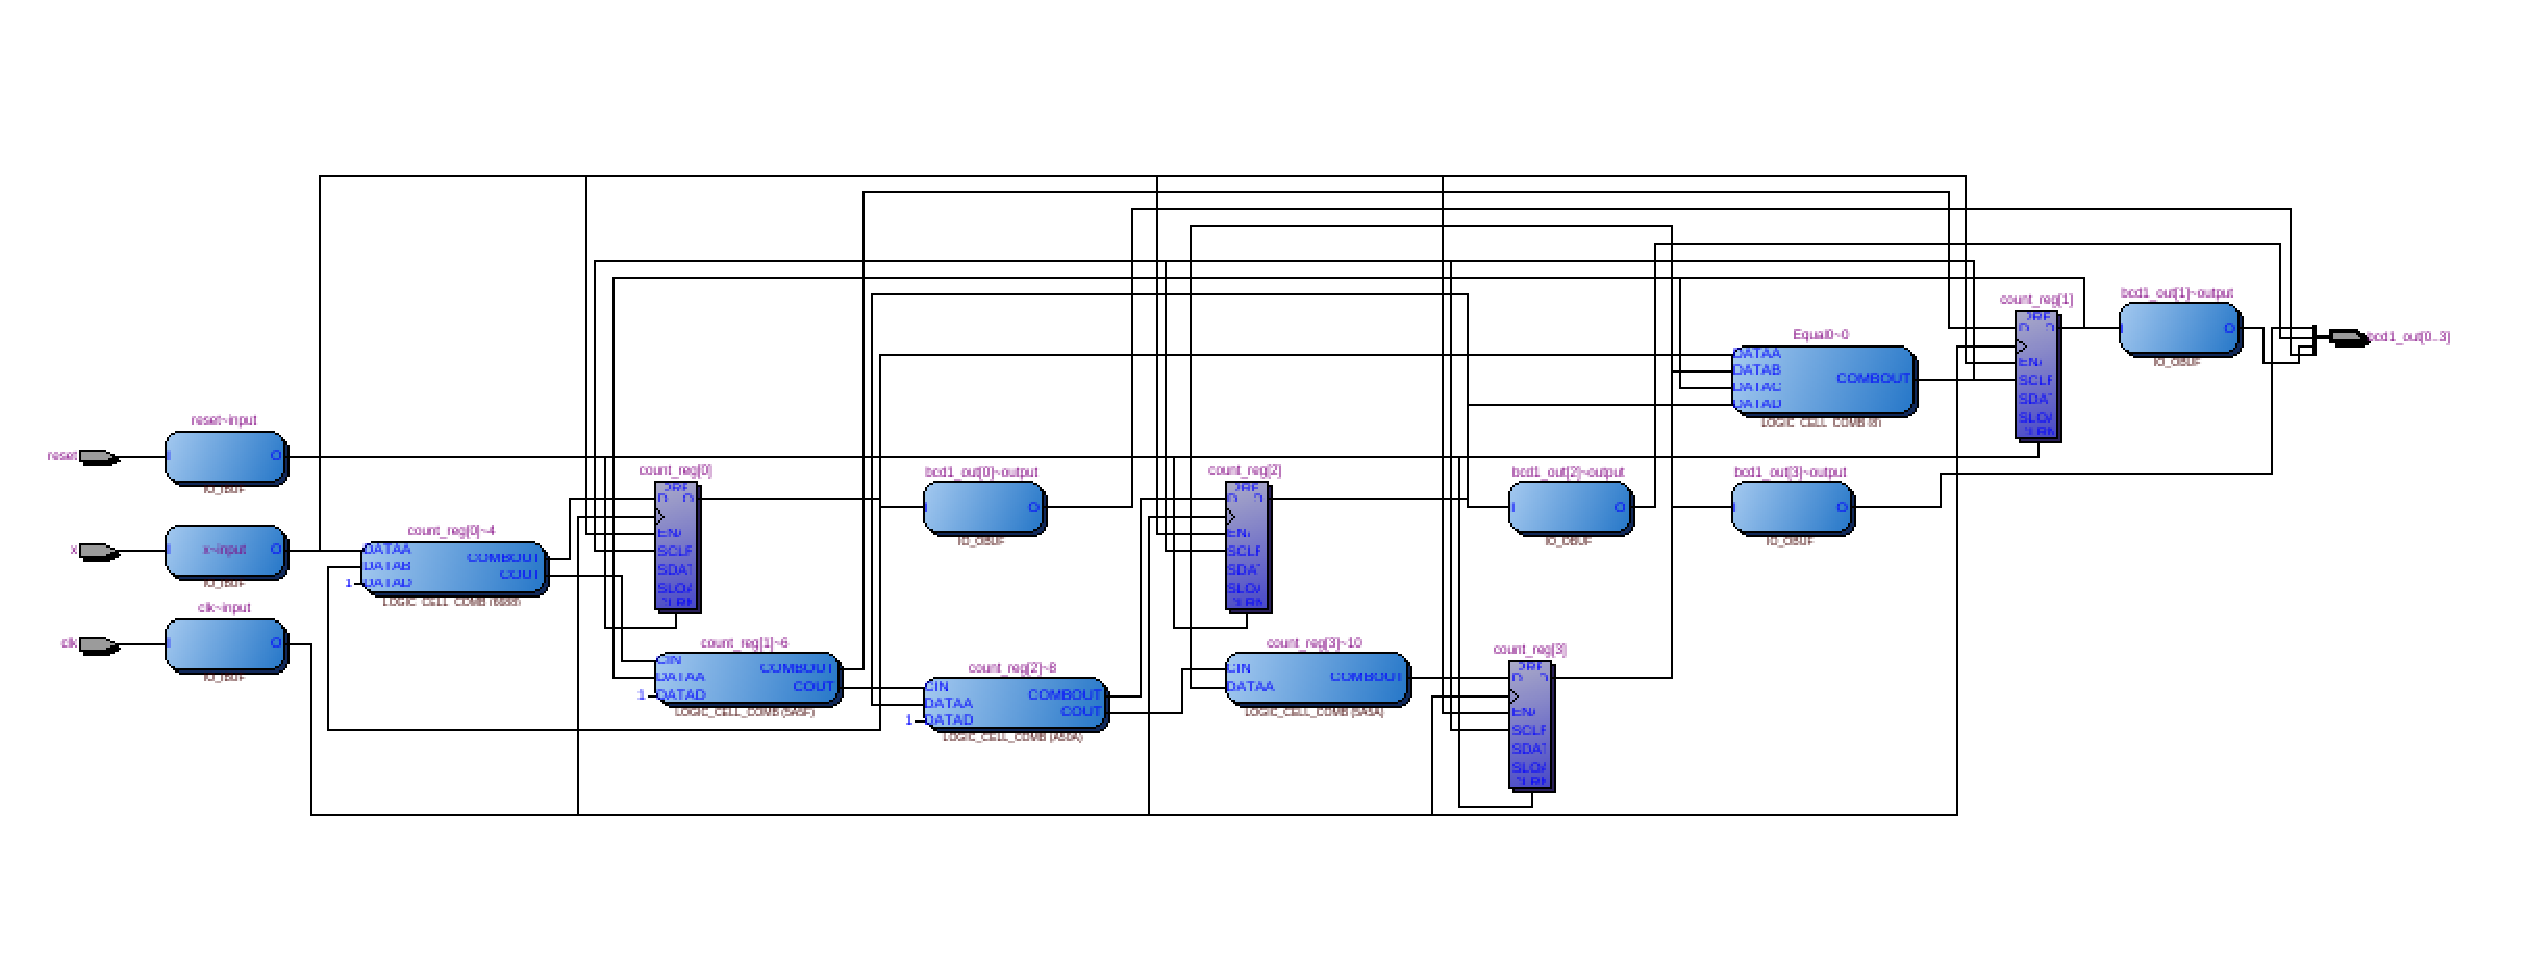
\includegraphics[width=13cm]{images/fig18.eps}
    \caption{1桁BCDカウンタ回路}
    \label{fig:18}
  \end{center}
\end{figure}

%---------------------------------------------------------------------
\subsection{考察}
%---------------------------------------------------------------------

考察は実験課題1の最後に1桁BCDカウンタ、2桁BCDカウンタともに考察する。

\clearpage

%===================================================================
\section{2桁BCDカウンタの階層設計(実験課題1)}
%===================================================================

%---------------------------------------------------------------------
\subsection{目的・概要}
%---------------------------------------------------------------------

今回の実験では、前述の1桁BCDカウンタを用いて2桁BCDカウンタを階層設計する。
この順序回路も同様にVerilog HDLで記述して、機能レベルシミュレーションにより動作を確認、
また、論理合成を実行して合成結果を確認する。

%---------------------------------------------------------------------
\subsection{実験手順}
%---------------------------------------------------------------------

今回の実験は、2桁のBCDカウンタの階層設計を行った。
仕様は以下の通りである。

\begin{itemize}
  \item 入力: クロックclk(1ビット), リセットreset(1ビット), カウントアップ信号x(1ビット)
  \item 出力: カウンタ値出力bcd2_out(8ビット)
  \item 機能: リセットが0になると出力の各ビットは0になる(非同期リセット)。出力値はclkが0から1に変化かつカウントアップ信号が1になるたびに
	         カウントアップし、0000 0000 -> 0000 0001 -> 0000 0010 -> ... -> 1001 1001 -> 0000 0000 -> 0000 0001 -> ...のようになる。
\end{itemize}


はじめに、Verilog HDLで順序回路記述した。そのコードは以下の通りである。

\lstinputlisting[caption=2桁BCDカウンタ,label=bcd2.v]{../../jikken-kadai1/bcd2.v}

このコードの構造を説明する。

\begin{itemize}
  \item 1~4行目はコメントである。
  \item 6行目で、前回設計した1桁BCDカウンタ{\tt bcd1.v}を読み込む記述をした。
  \item 8行目から{\\ bcd2}のモジュールを記述した。
  \item 9, 10行目で入出力の設定をした。
  \item 13~16行目、19~22行目で出力を観測するための信号線を宣言した。
  \item 25, 26行目で、入力のクリック信号を{\tt bcd1a, bcd1b}に代入する記述をした。
  \item 29, 30行目で、入力のリセット信号を{\tt bcd1a, bcd1b}に代入する記述をした。
  \item 33行目で入力の{\tt x}を{\tt bcd1a}のカウントアップ信号へ代入する記述をした。
  \item 36, 37行目で{\tt bcd1a, bcdab}の実体化を記述した。引数は1桁BCDカウンタの時と同様で、クリック信号clk、リセット信号reset, 
	  とカウントアップ信号xと{\tt bcd1a\_out}で4ビット出力を当てている。{\tt bcd1b}についても同様。
  \item 40行目で2桁目のカウントアップ信号を制御す記述を行った。
          1桁目が9の時に2桁目がカウントアップされればいいので、{\tt bcd1a\_out == 9}の時に{\tt bcd1b\_x}に1を代入させた
	  この論理式も10進数で{\tt == 9}としても、1桁ずつ判定を行っても結果は同じなので、より読解性の高い記述を選んだ。
  \item 43行目で2桁BCDカウンタの出力をビット連接で8ビットにして行った。
\end{itemize}

続いて、2桁BCDカウンタを動かすためのテストベンチを作成した。

\lstinputlisting[caption=2桁BCDカウンタのテストベンチ,label=test_bcd2.v]{../../jikken-kadai1/test_bcd2.v}

ただし、このテストベンチは1桁BCDカウンタと動作の仕組みは同様であるので、プログラムの説明は省略する。

%---------------------------------------------------------------------
\subsection{実験結果}
%---------------------------------------------------------------------

%----------------------------------
\subsubsection{機能レベルシミュレーション}
%----------------------------------

図\ref{fig:19}に示す波形を得た。

\begin{figure}[htb]
  \begin{center}
    \includegraphics[width=13cm]{images/fig19.eps}
    \caption{機能レベルシミュレーションを行った結果の波形}
    \label{fig:19}
  \end{center}
\end{figure}

%----------------------------------
\subsubsection{論理合成}
%----------------------------------


コンパイル結果のロジックエレメント数は図\ref{fig:20}のようだった。
ロジックエレメント数は\ref{fig:20}のTotal Logic Elementの部分である。  

\begin{figure}[htb]
  \begin{center}
    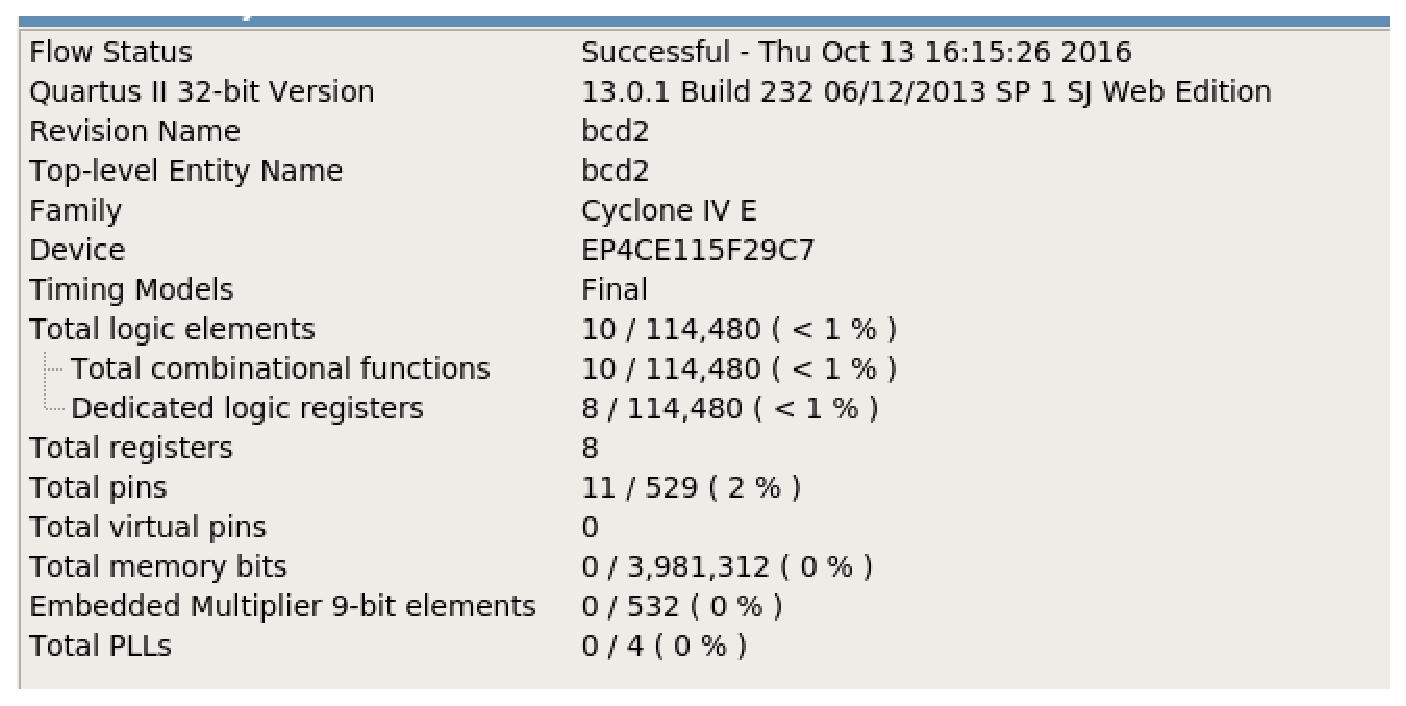
\includegraphics[width=13cm]{images/fig20.eps}
    \caption{ロジックエレメント数}
    \label{fig:20}
  \end{center}
\end{figure}

回路の遅延時間は図\ref{fig:21}の通りだった。
トータルの遅延時間はここでは、5.131nsとなる。

\begin{figure}[htb]
  \begin{center}
    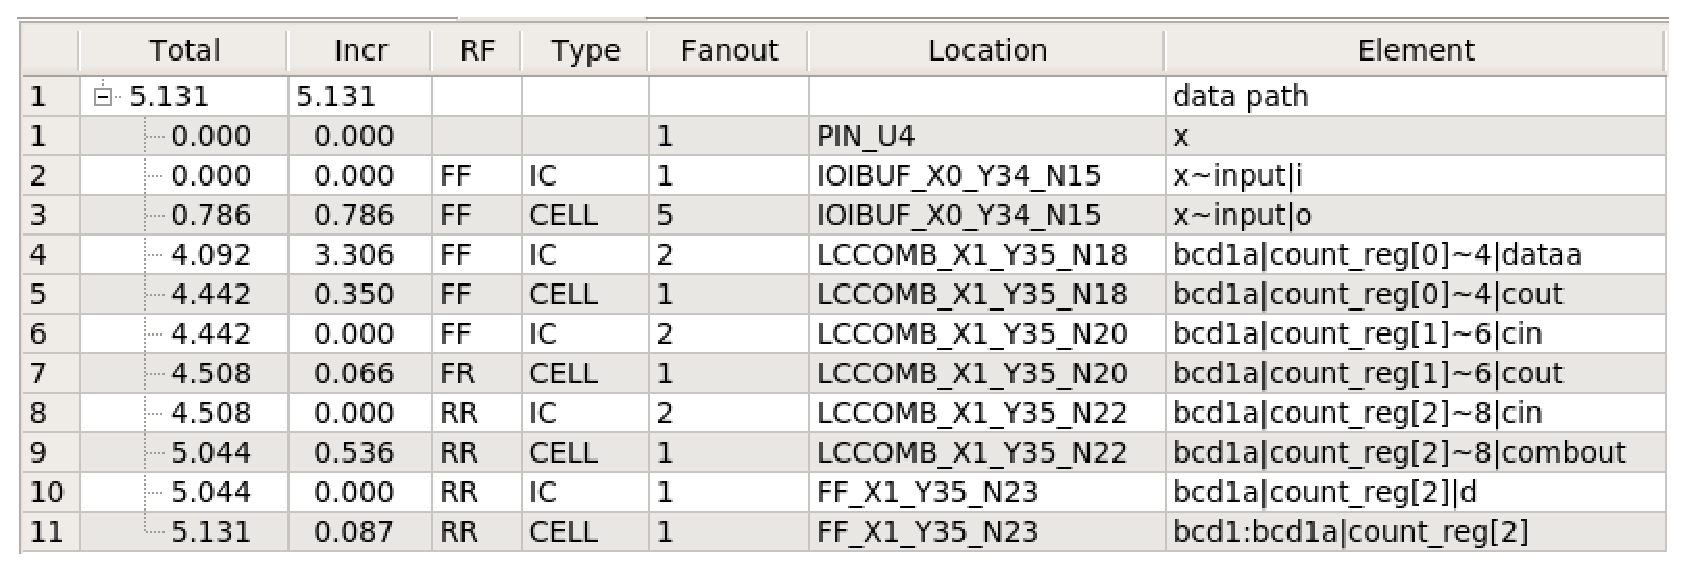
\includegraphics[width=13cm]{images/fig21.eps}
    \caption{遅延時間}
    \label{fig:21}
  \end{center}
\end{figure}

最適化後の回路は図\ref{fig:22}の通りだった。

\begin{figure}[htb]
  \begin{center}
    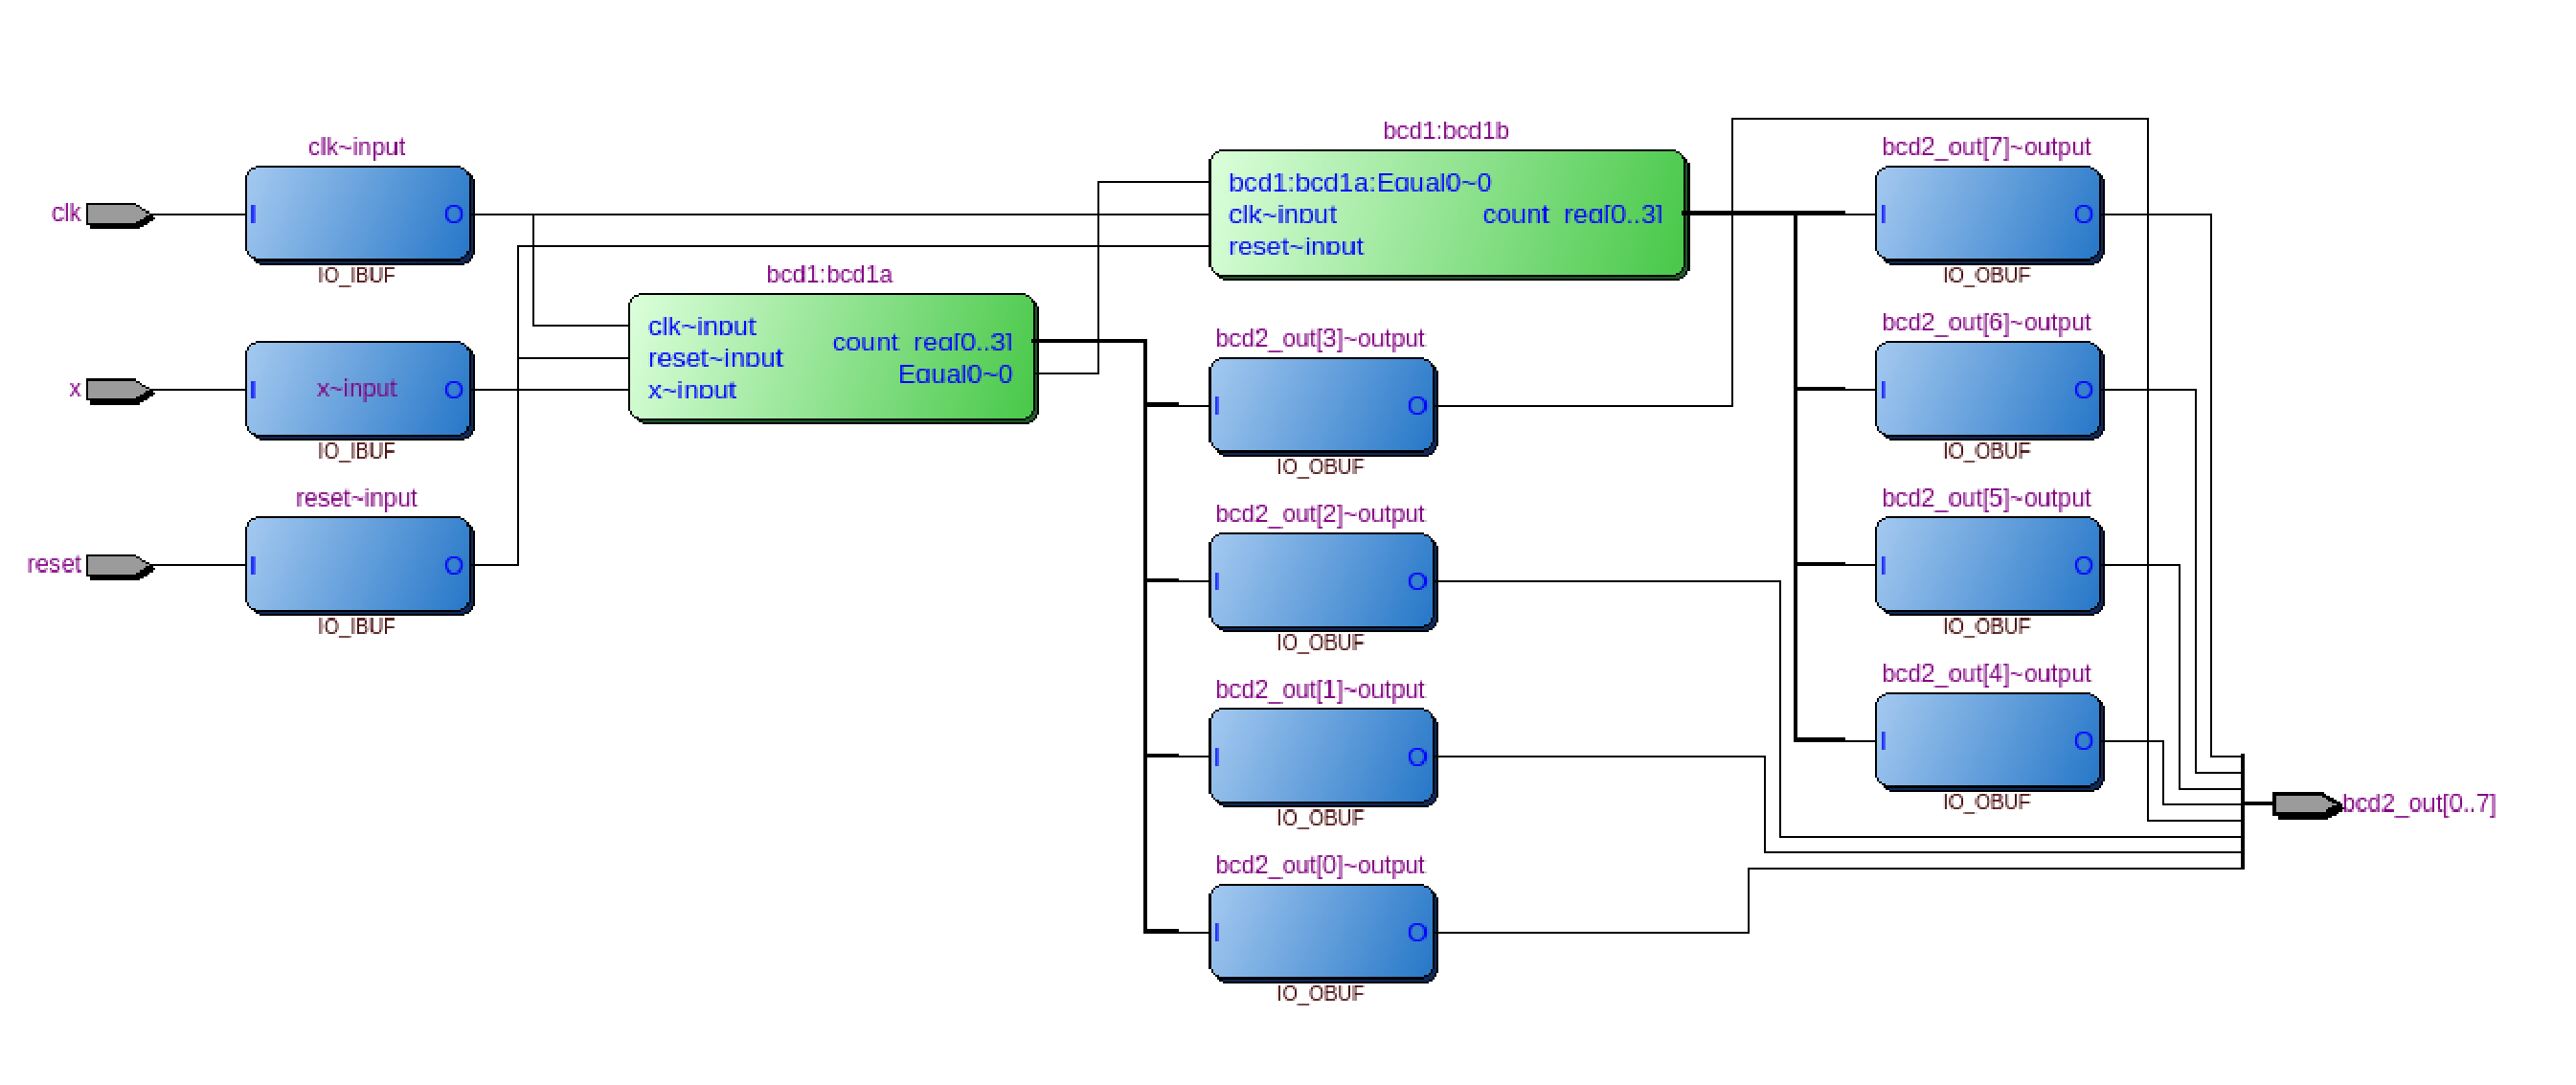
\includegraphics[width=13cm]{images/fig22.eps}
    \caption{2桁BCDカウンタ回路}
    \label{fig:22}
  \end{center}
\end{figure}

%---------------------------------------------------------------------
\subsection{考察}
%---------------------------------------------------------------------

1桁BCDカウンタ回路とそれを用いて階層設計した2桁BCDカウンタ回路では、2桁BCDカウンタは
1桁BCDカウンタを2つ用いたのでレジスタ数やロジックエレメント数は論理合成の結果もちろん倍になっていたが、
そこに使用されているピンの数は2桁BCDカウンタ回路になることで割合が減っていた。これは順序回路で設計
したことで、回路が小さくなったことによると推測される。

実際に遅延時間に関しても、1桁BCDカウンタでは5.169nsで2桁BCDカウンタでは5.131nsとなっている。このように
順序回路は設計はレジスタや制御回路が必要なので、設計が複雑になり、バグの混入やミスにつながるデメリットはあるが、
うまく設計すると結果的に回路が小さくなることで、内部的な遅延時間が減少するメリットがあると推測される。

\clearpage

%===================================================================
\section{系列検出回路の設計(実験課題2)}
%===================================================================

%---------------------------------------------------------------------
\subsection{目的・概要}
%---------------------------------------------------------------------

今回の実験では、系列検出回路(有限オートマトン)の設計を状態機械による順序回路記述によって行う。
この順序回路を同様にVerilog HDLで記述して、機能レベルシミュレーションにより動作を確認、
また、論理合成を実行して合成結果を確認する。

%---------------------------------------------------------------------
\subsection{実験手順}
%---------------------------------------------------------------------

今回の実験は、0011および0010という入力系列を入力される後とに1を出力する系列検出回路の設計を行う。
仕様は以下の通りである。

\begin{itemize}
  \item 入力: クロックclk(1ビット), リセットreset(1ビット), データ入力x(1ビット)
  \item 出力: 検出結果出力y(1ビット)
  \item 機能: リセットが0になると出力は0になる(非同期リセット)。出力値は、0011または0010という系列を検出したときのみ1になる。
\end{itemize}

はじめに、Verilog HDLで順序回路記述した。そのコードは以下の通りである。

\lstinputlisting[caption=系列検出回路,label=m.v]{../../jikken-kadai2/m.v}

このコードの構造を説明する。

\begin{itemize}
  \item 1~4行目で、4つの状態の値を定義した。{\tt st0, st1, st2, st3}の順に2進数で{\tt 00, 01, 10, 11}とした。
  \item 6行目でモジュールブロックを記述した。
  \item 7, 8行目で入出力を設定した。
  \item 10行目で出力値を記憶しておく1ビットレジスタを宣言した。
  \item 11行目で状態を記憶しておく2ビットレジスタを宣言した。
  \item 13行目で出力{\tt y}に出力レジスタの値を代入した。
  \item 15行目から、{\tt always}ブロックの記述をした。{\tt always}ブロックの発生条件は、クロックの立ち上がりとリセット信号の立ち下がりである。
  \item 18,19行目で{\tt reset == 1}のときに、つまり、リセット信号を検出している時にレジスタが初期化されるように記述した。
  \item 21~56行目には、状態遷移の記述を行った。状態はレジスタ{\tt st\_reg}に記憶してあり、その値によって{\tt case}構文によって分岐したそれぞれの状態において、入力値{\tt x}の条件分岐によって{\tt st\_ref, y\_reg}を状態遷移図にあわせて変化する記述を行った。
\end{itemize}

続いて、系列検出回路を動かすためのテストベンチを作成した。

\lstinputlisting[caption=系列検出回路のテストベンチ,label=test_m.v]{../../jikken-kadai2/test_m.v}

このコードの構造を説明する。

\begin{itemize}
  \item 1~4行目はコメントである。
  \item 6,7行目でシミュレーションの単位時間/精度の宣言と、m.vを読み込んだ。
  \item 9行目から、モジュールブロックを宣言した。
  \item 11行目で、{\tt m}の入力値を格納するレジスタ{\tt reset, clk, x}(各々1ビット)を宣言した。
  \item 14行目で、出力を観測するための信号線{\tt y}を宣言した。
  \item 17行目で、{\tt m}を実体化する処理を記述した。
  \item 19~21行目で、5nsごとにクリック信号を送る記述をした。これは{\tt clk}を反転することで実現している。
  \item 23~42行目はテストの本体で、まず初めに{\tt reset=0; clk=0; x=0}と初期値を設定した。
	  リセット信号は20ns後に{\tt 0}に、その次の20ns後に{\tt 1}に戻る処理を記述した。次に系列{\tt 1001110}を10ns刻みに
	 次々と入力した。そのさらに1000ns後にテストベンチを終了する記述をした。
\end{itemize}

%---------------------------------------------------------------------
\subsection{実験結果}
%---------------------------------------------------------------------

%----------------------------------
\subsubsection{機能レベルシミュレーション}
%----------------------------------

図\ref{fig:23}に示す波形を得た。

\begin{figure}[htb]
  \begin{center}
    \includegraphics[width=13cm]{images/fig23.eps}
    \caption{機能レベルシミュレーションを行った結果の波形}
    \label{fig:23}
  \end{center}
\end{figure}

%----------------------------------
\subsubsection{論理合成}
%----------------------------------


コンパイル結果のロジックエレメント数は図\ref{fig:24}のようだった。
ロジックエレメント数は\ref{fig:24}のTotal Logic Elementの部分である。  

\begin{figure}[htb]
  \begin{center}
    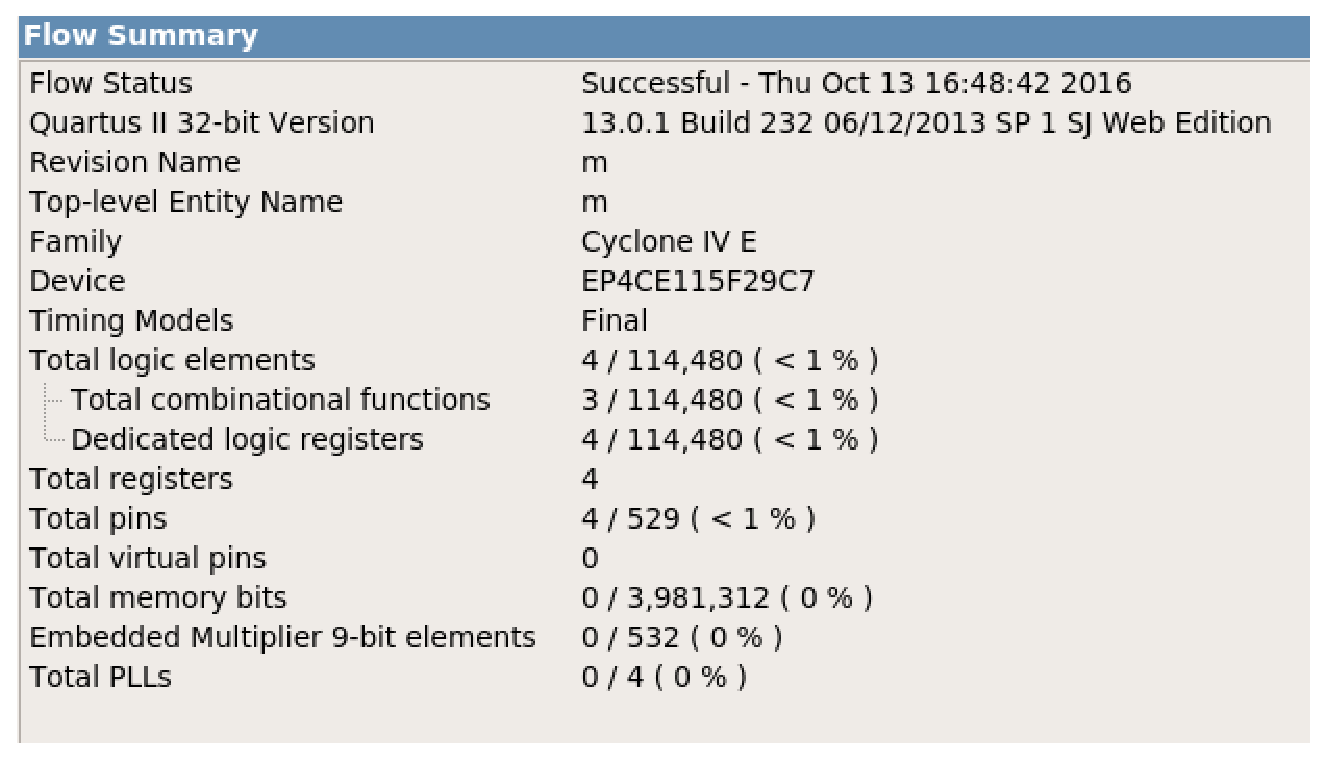
\includegraphics[width=13cm]{images/fig24.eps}
    \caption{ロジックエレメント数}
    \label{fig:24}
  \end{center}
\end{figure}

回路の遅延時間は図\ref{fig:25}の通りだった。
トータルの遅延時間はここでは、4.357nsとなる。

\begin{figure}[htb]
  \begin{center}
    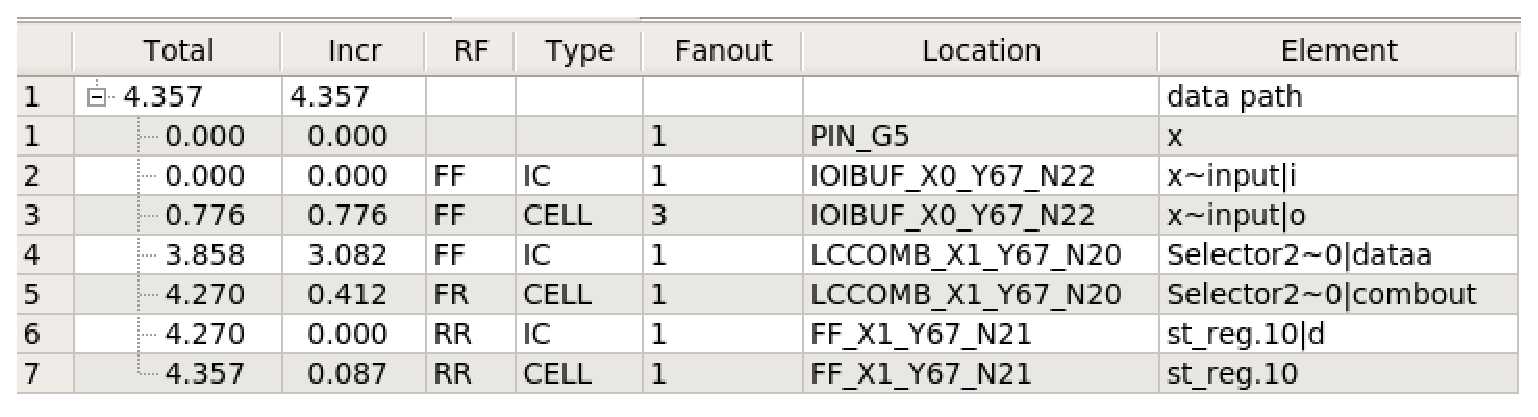
\includegraphics[width=13cm]{images/fig25.eps}
    \caption{遅延時間}
    \label{fig:25}
  \end{center}
\end{figure}

最適化後の回路は図\ref{fig:26}の通りだった。

\begin{figure}[htb]
  \begin{center}
    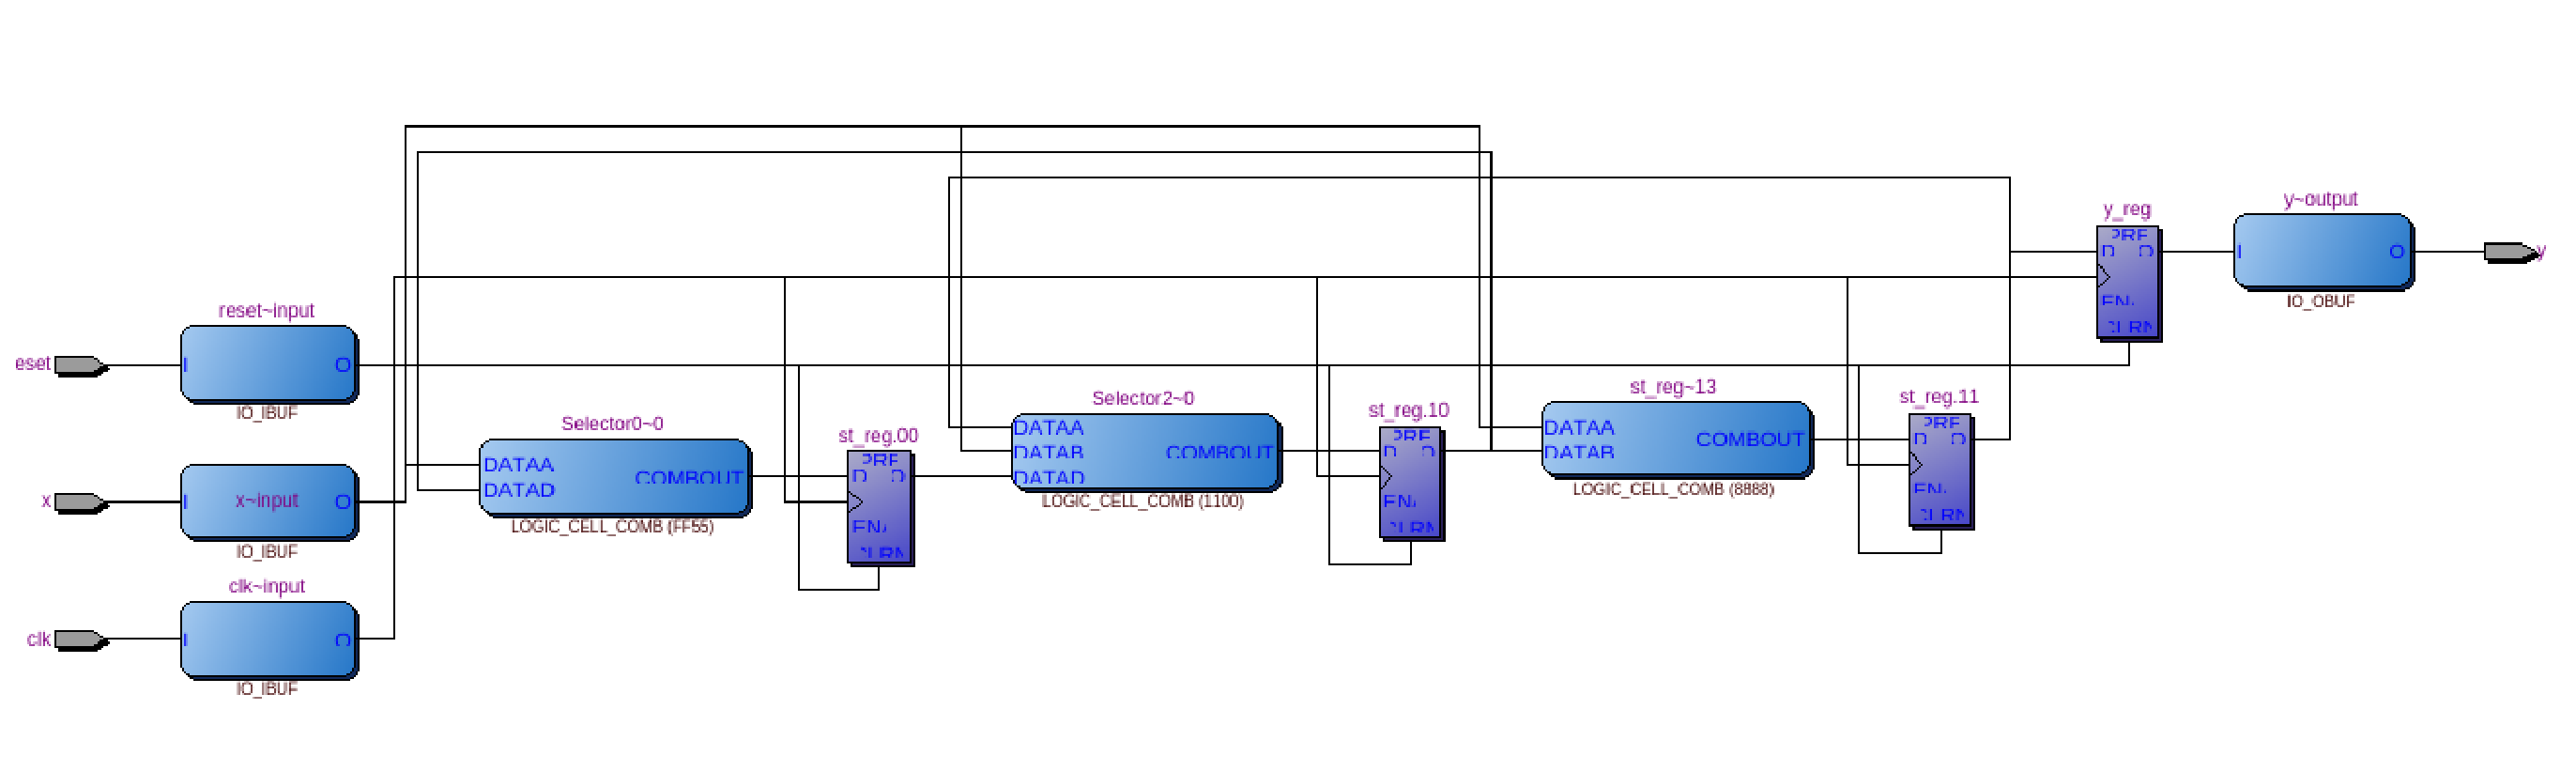
\includegraphics[width=13cm]{images/fig26.eps}
    \caption{系列検出回路}
    \label{fig:26}
  \end{center}
\end{figure}


%---------------------------------------------------------------------
\subsection{考察}
%---------------------------------------------------------------------

図\ref{fig:23}からも入力系列{\tt 1001110}のうち、{\tt 0010}を検出してそこで1を出力していることが確認できる。

今回は状態遷移図として{\tt st0, st1, st2, st3}を以下のような状態と定義していた。

\begin{table}[htb]
  \begin{tabular}{lcrr}
    	状態名 & 状態
	st0 & 何も入力されていない \\
     	st1 & 0を検知  \\
	st2 & 00を検知 \\
	st3 & 001を検知 \\
  \end{tabular}
\end{table}

なので、もし系列{\tt 0010011}がきた場合、今回の設計だと前半の{\tt 0010}を検出して1をそこで出力し、
その後に続いて{\tt 0011}も検出して、またここで1を出力する設計になっている。

これは{\tt st3}の状態で入力が{\tt 0}でも{\tt 1}でも、{\tt 0010, 0011}に引っかかるので1を出力するが、
ここで{\tt 0}がきた場合に、{\tt 1}がきた時と同様に{\tt st0}に遷移するのではなく、引き続き{\tt st1}に
遷移するようにしたからである。
ここで{\tt 1}がきた時と同様に{\tt 0010, 0011}のいずれかを検出したら{\tt st0}にもどると言う設計に
すれば今の入力系列では1は一回しか出力されない。ただし、今回はその設計にはしなかった。

\clearpage

%===================================================================
\section{16ビット加算回路の実現方法による比較}
%===================================================================

この節では主に,参考文献\cite{altera}を参考に記述している.

%---------------------------------------------------------------------
\subsection{はじめに}
%---------------------------------------------------------------------

実験2と実験3では、16ビット加算回路を組み合わせ回路で実現する方法と順序回路で実現する方法をためした。この論理合成の結果を比較し、考察しろ。

実験2で設計した16ビット加算回路は組み合わせ回路のみで設計されていて、入力に対して即時に出力が決まるというシンプルな構成となっている。
一方、実験3で設計した16ビット加算回路は順序回路といって組み合わせ回路+記憶回路からなっている。
この2種類の実現方法による論理合成の結果を比較する。

%---------------------------------------------------------------------
\subsection{考察}
%---------------------------------------------------------------------

実験2の論理合成の結果である図\ref{fig:07}, \ref{fig:08}と実験3の\ref{fig:12}, \ref{fig:13}を比較してみる。

実験2の組み合わせ回路はレジスタを用いないのでロジックエレメント数は、レジスタを必要な実験3のそれよりも少なくて済んでいる。
しかし、遅延時間を見ると、ロジックエレメント数の多い実験3の回路の方が短くなっていることが分かる。

この事から、順序回路ではレジスタや制御回路が必要なため、複雑な回路になるため設計に時間がかかったりバグが混入しやすくなる
というデメリットはあっても、結果的に回路が小さくなる事が推測される。

例えば、加算器を例にとると、組み合わせ回路で設計した場合、全加算器が桁数だけ必要になる(2ビット加算器では2個のように)。
しかし、順序回路では全加算器をたったの1個で実現できる。このためそこからの出力を保持しておくためにレジスタや制御回路が
必要となるが、これは桁数が増えれば増えるほど得られるメリットは大きいと推測される。

また、順序回路は一般的に動作が遅いと言われているが、確かに逐次処理は遅くなってしまう。しかし、順序回路=低速とは限らない場合も多々ある。
再び加算器の例で行くと、一度に計算するビット数を増やすことで処理を並列化し、処理時間を短くすることができる。ただし、この場合では、計算する回路
の面積(この例だと、全加算器の個数)が増加するため、面積と処理時間はトレードオフの関係にある。

\clearpage

%===================================================================
\section{論理回路の最適化について}
%===================================================================

この節では主に,参考文献\cite{siba}を参考に記述している.

%---------------------------------------------------------------------
\subsection{最適化の目的と指針}
%---------------------------------------------------------------------

論理回路の最適化が必要な理由は「論理回路を論理ゲートや配線という基本部品によって構成する」からである.
論理ゲートの個数が減り,配線が簡単になると以下のようなメリットがある.

\begin{enumerate}
  \item 論理回路の実装コストが安くなる.
  \item 論理回路の耐故障性が増す.
\end{enumerate}

論理ゲートを論理回路の構成用部品として用いるには,必要な空間や時間の大きさに配慮した設計が必要となる.
論理回路の最適化設計に対する指標は次の2種類がある.

\begin{description}
 \item[空間最適化]\mbox{}\\
   論理回路を構成するのに必要なゲートの総数を最小にする.
 \item[時間最適化]\mbox{}\\
  論理回路の入力端子から出力端子に至までに通過する論理ゲートの段数\footnote{論理回路の入力端子から出力端子に至るまでに通過する論理ゲート数のこと}を最小にする.
  入力端子から出力端子に至るまでの経路は普通複数あるが,時間最適化では,このうち最も多い段数の経路の段数を最小にする.
\end{description}

\subsection{最適化設計の手法}

一般的に,任意の論理関数に対応する論理回路が存在し,逆に,任意の論理回路は論理関数によって表現できることが分かっている.
論理回路図が与えられていて,それをもとにその論理回路を表現する論理関数をもとめることを「論理回路の{\bf 解析}」という.
逆に,論理関数が与えられていて,それをもとにその論理関数に対応する論理回路を求めることを「論理回路の{\bf 解析}あるいは{\bf 合成}」という.

論理回路における論理ゲートは論理関数における論理演算に対応している.
従って,論理ゲートの個数を減らすためには,対応する論理演算の個数を減らせばよい.

最適化設計の手法としては,主に次のようなものが挙げられる.

\begin{description}
 \item[論理関数と論理回路の最小化]\mbox{}\\ 
  論理関数の最適化と論理回路の最適化は連動しているので,論理関数を最小化する.
 \item[カルノー図による2段階論理最小化]\mbox{}\\
  論理関数の表現法の1つであるカルノー図を用いて組み合わせ回路を直感的に最適化設計する.
 \item[クワイン-マクラスキ法による2段階論理最小化]\mbox{}\\
  論理関数の真理値表表現をもとにして,それを併合・簡単化することによって,論理最小化を図る.
 \item[論理式の変形による多段論理最小化]\mbox{}\\
  論理式から共通項をくくり出す操作を行う.
\end{description}

\subsection{最適化された論理回路の遅延時間と面積の関係}

論理合成から所望の回路を出力させるにはHDLを適切に記述する他に,合成される回路の面積や速度といった制約条件が適切でなければならない.
設計する上で考慮しなけらばならない2つの制約を挙げる.

\begin{description}
 \item[エリア制約]\mbox{}\\ 
   回路の面積やゲート数の制約のこと.
 \item[タイミング制約]\mbox{}\\
  クロック周期と回路の出力ポートに対する最大遅延,最小遅延の制約のこと.
\end{description}

この2つの制約にはトレードオフの関係がある(図\ref{fig:03}).

\begin{figure}[htb]
  \begin{center}
    \includegraphics[width=8cm]{images/fig-03.eps}
    \caption{面積とディレイのトレードオフ}
    \label{fig:03}
  \end{center}
\end{figure}

\begin{thebibliography}{99}
\bibitem{hdl} 深山 正幸・北川 章夫・秋田 純一・鈴木 正國 著, 『HDLによるVLSI設計―VerilogHDLとVHDLによるCPU設計― 第2版』,共立出版(2002年)
\bibitem{siba} 柴山 潔 著, 『コンピュータサイエンスで学ぶ 論理回路とその設計』,近代科学社(1999年)
\bibitem{et01} ``Combinational Logic Circuits using Logic Gates'', \url{http://www.electronics-tutorials.ws/combination/comb_1.html}
\bibitem{altera} 順序回路は組合せ回路を記述できる!? ,\url{http://www.hirokinakaharaoboe.net/tips_wiki/index.php?%E9%A0%86%E5%BA%8F%E5%9B%9E%E8%B7%AF%E3%81%AF%E7%B5%84%E5%90%88%E3%81%9B%E5%9B%9E%E8%B7%AF%E3%82%92%E8%A8%98%E8%BF%B0%E3%81%A7%E3%81%8D%E3%82%8B%EF%BC%81%EF%BC%9F%E3%80%90Altera%20DE0%E3%80%91}
\end{thebibliography}

\clearpage

\appendix

\end{document}


